\documentclass[11pt,a4paper,openany]{report}
\usepackage[T1]{fontenc}
\usepackage[utf8]{inputenc}
\usepackage{lmodern}
\usepackage{microtype}
\usepackage{amsmath,amssymb,amsthm,mathtools,bm}
\usepackage{booktabs,array,longtable,tabularx}
\usepackage{xcolor}
\usepackage[margin=24mm,headheight=23pt]{geometry}
\usepackage{enumitem}
\usepackage{fancyhdr}
\usepackage{fancyvrb}
\usepackage{graphicx}
\usepackage{url}
\usepackage{xurl}
\usepackage{hyperref}

\definecolor{finblue}{HTML}{1F5A99}
\definecolor{fingreen}{HTML}{19733A}
\definecolor{finorange}{HTML}{D55E00}
\definecolor{finred}{HTML}{A61B1B}
\definecolor{finviolet}{HTML}{6A3D9A}

\hypersetup{
  unicode=true,
  colorlinks=true,
  linkcolor=finblue,
  citecolor=fingreen,
  urlcolor=finblue,
  pdftitle={FIN Programs 191--203: Reference States, Operational Quotients, and Conditional Prediction},
  pdfauthor={Krzysztof Żuchowski},
  pdfsubject={Reference-state naturality, scale quotients, reflection conversion, process tomography, environment identifiability and conditional prediction},
  pdfkeywords={FIN, operator algebra, spectral theory, Dirichlet form, Alberti-Uhlmann, process tensor, mixing, operational physics, scale quotient}
}

\pagestyle{fancy}
\fancyhf{}
\fancyhead[L]{\small FIN Programs 191--203}
\fancyhead[R]{\small Release 10.18}
\fancyfoot[C]{\thepage}
\setlength{\parindent}{0pt}
\setlength{\parskip}{0.55em}
\setlist{nosep,leftmargin=2em}
\setcounter{tocdepth}{2}
\setcounter{secnumdepth}{3}
\emergencystretch=3em

\newcommand{\one}{\bm 1}
\newcommand{\C}{\mathbb C}
\newcommand{\R}{\mathbb R}
\newcommand{\Z}{\mathbb Z}
\newcommand{\statusProven}{\textcolor{fingreen}{[Proven]}}
\newcommand{\statusComputer}{\textcolor{fingreen}{[Proven, computer-assisted]}}
\newcommand{\statusStrong}{\textcolor{finblue}{[Strong evidence]}}
\newcommand{\statusConditional}{\textcolor{finorange}{[Conditional]}}
\newcommand{\statusRefuted}{\textcolor{finred}{[Refuted in scope]}}
\newcommand{\statusOpen}{\textcolor{finviolet}{[Open]}}

\begin{document}
\hypersetup{pageanchor=false}
\begin{titlepage}
\centering
\vspace*{8mm}
{\Large\bfseries FIN Research Monograph --- Release 10.18\par}
\vspace{10mm}
{\Huge\bfseries FIN Programs 191--203\par}
\vspace{6mm}
{\Large Reference States, Operational Quotients,\\
and Conditional Prediction\par}
\vspace{16mm}
{\Large Krzysztof \.Zuchowski\par}
\vspace{2mm}
{\normalsize Independent Researcher --- Fractal Information Theory Project\par}
\vspace{2mm}
{\normalsize ORCID: \href{https://orcid.org/0009-0002-0909-3613}{0009-0002-0909-3613}\par}
\vspace{10mm}
{\large 27 July 2026\par}
{\normalsize Publication --- Preprint; record version 1.0.0\par}
\vfill
\begin{minipage}{0.88\textwidth}
\small
\textbf{Scope.} Thirteen executed studies of reference-state naturality,
compression gauge, rigorous certification, finite Dirichlet dynamics,
reflection-covariant conversion, mixing-aware inference, temporal open-set
detection, process tomography, environment equivalence, analytic phase
provenance, scale-free observables, experimental intake and one conditional
prediction.

\medskip
\textbf{Central result.} The qubit reflection-conversion boundary is reduced
to a finite closed formula, and single/plus/echo process tomography is proven
minimal for an unknown-blur Gaussian two-step model. States on non-simple
algebras, positive scale and microscopic environments remain nontrivial
moduli or quotient data.

\medskip
\textbf{Guardrail.} No QW-2191 discharge, strict selector, physical unit,
strict beta source, completed legacy--strict bridge, role transfer,
\(L_{\rm total}\), Theory-of-Everything closure or external physical
validation is claimed.

\medskip
\textbf{License.} Creative Commons Attribution 4.0 International (CC BY 4.0).
\end{minipage}
\vfill
\end{titlepage}
\hypersetup{pageanchor=true}

\pagenumbering{roman}
\chapter*{Publication statement}
\addcontentsline{toc}{chapter}{Publication statement}
This release reports Programs 191--203 and recommends Programs 204--216.
Analytic proofs, exact finite audits, synthetic evidence, conditional
constructions, unavailable proof toolchains and external-data failures are
kept separate.

\tableofcontents
\clearpage
\pagenumbering{arabic}

\section{Confidence convention}

The report distinguishes analytic proof, exact finite computation, synthetic evidence, conditional construction and open obligations. No unavailable certificate is promoted by prose.

\chapter{Abstract}

This monograph reports thirteen executed research programs, numbered 191 through 203, concerning the mathematical and operational completion of the dimensionless FIN spectral framework. The studies were selected by the previous Programs 178--190 round. They address reference-state naturality, compression-scale gauge reduction, rigorous numerical certification, finite Dirichlet dynamics, reflection-covariant state conversion, dependent-data inference, temporal open-set detection, process-tensor tomography, environmental nonidentifiability, analytic phase provenance, scale-free observables, experimental data intake, and one conditional prediction pipeline.

Four theorem-level advances are obtained.

First, invariant states on a finite direct sum

\[
\mathcal A=\bigoplus_i M_{d_i}(\mathbb C)
\]

are classified. Inner-unitary naturality uniquely fixes normalized trace on each simple block but leaves a probability measure on the centre. For the FIN dimension vector \((1,2,2,2,2)\), uniform central weighting gives \(9/5\) whereas the normalized full trace gives \(17/9\). Neither value is selected without an additional central-measure principle.

Second, the positive compression parameter is quotiented by its length-scale action. The complete amplitude-normalized orbit representative is

\[
\widehat K(x)=
\frac{\cos(\nu x+\phi)}{1+x^\eta},
\qquad
x=\beta^{1/\eta}d,
\qquad
\nu=\frac{\omega}{\beta^{1/\eta}}.
\]

This proves that \(\beta=1\) is a coordinate representative, while \((\eta,\nu,\phi)\) remain gauge-invariant. The legacy and strict kernels remain strongly separated after quotienting; the scale gauge therefore does not complete their bridge.

Third, the numerical maximization in the complete one-qubit reflection-covariant conversion criterion is eliminated. An Alberti--Uhlmann reduction gives a closed boundary determined by only three candidate points. For source \((r_s,z_s)\) and prescribed target \(z_t\),

\[
r_{t,\max}^2
=
\min_{x\in\{0,1,x_c\}}
\left[
\max\{x,r_s^2+xz_s^2\}-xz_t^2
\right],
\qquad
x_c=\frac{r_s^2}{1-z_s^2}.
\]

The previous equal-monotone counterexample is recovered exactly: \((0.6,0)\to(0.6,0.8)\) is impossible because \(r_{t,\max}=0.36\).

Fourth, a minimal three-contrast process-tomography frame is proved for a two-step Gaussian dephasing process with unknown detector blur. Single, plus, and echo visibilities form a rank-three log-linear system identifying blur, increment variance, and temporal covariance. Removing the echo contrast lowers the rank to two.

The round also constructs a valid nonasymptotic DKW procedure for an observed regenerative beta-mixing acquisition class, a preregistered order-sensitive open-set detector, an operational environment quotient, a no-go theorem for natural analytic legacy-to-strict phase generation, and the projective algebra of scale-free spectral observables.

Two requested closure tasks remain honestly blocked: Arb/\allowbreak{}python-flint is not available for the common directed-rounding certificate, and no local Lean toolchain compiles the supplied finite Dirichlet library. A complete event-level synthetic bundle validates ten of eleven intake fields but fails the independent-analysis boundary. Consequently the final \(W_0+\mathrm{CA}+\mathrm{OP}\) prediction is executed only as a synthetic dry run and is not described as external physics.

No non-premise selector, physical unit, target-independent strict compression source, completed legacy-to-strict bridge, legacy role transfer, role-bearing \(L_{\rm total}\), experimentally validated physical claim, or Theory-of-Everything closure is asserted.

\par\medskip\hrule\medskip

\chapter{Executive summary}

\section{The outcome}

The round replaces several informal "missing constant" questions by typed mathematical objects.

\begin{center}
\begingroup\small
\setlength{\tabcolsep}{3.5pt}
\renewcommand{\arraystretch}{1.16}
\begin{longtable}{@{}p{0.152\textwidth}p{0.384\textwidth}p{0.186\textwidth}p{0.139\textwidth}@{}}
\toprule
\textbf{Problem} & \textbf{Constructed object} & \textbf{Result} & \textbf{Confidence} \\
\midrule
\endhead
reference state & CentralMeasureFunctor & simple blocks fixed; central measure free & Proven \\
positive compression scale & BetaGaugeQuotient & \(\beta\) removed; shape mismatch survives & Proven \\
fractional certificate & CertificateDependencyDAG & one-engine certificate still unavailable & Proven audit \\
finite dual dynamics & FiniteDirichletCertificate & general proof and 150 exact checks; Lean uncompiled & Proven, compilation open \\
reflection conversion & AlbertiUhlmannReflectionCone & closed analytic boundary & Proven \\
dependent inference & ObservedRegenerationFrame & conditional DKW with random effective size & Proven \\
temporal open set & order-sensitive protocol & all four temporal challenges rejected in simulation & Strong evidence \\
process tomography & GaussianTwoStepTomographyFrame & three contrasts are necessary and sufficient & Proven in model \\
environment & OperationalEnvironmentQuotient & same channel can hide different processes & Proven \\
analytic phase source & PhaseSourceNaturalityNoGo & natural classes fail; successes are target-coded & Proven in classes \\
pre-clock observables & ProjectiveSpectralObservableAlgebra & invariant catalogue constructed & Proven \\
experimental intake & schema instance & synthetic 10/\allowbreak{}11; external gate fails & Proven audit \\
conditional prediction & ConditionalGaussianVisibilityLaw & held-out synthetic residual \(0.03646\) & Strong method evidence \\
\bottomrule
\end{longtable}
\endgroup
\end{center}

\section{The central scientific conclusion}

The single self-adjoint spectral generator still unifies wave, diffusion, and Green dynamics:

\[
U_t=e^{-itA},
\qquad
P_t=e^{-tA},
\qquad
G_z=(A+zI)^{-1}.
\]

But it does not uniquely determine:

\begin{itemize}
\item 
a state on a non-simple algebra;

\item 
a representative of the positive scale orbit;

\item 
an environment inside a reduced-process equivalence class;

\item 
a preparation or intervention family;

\item 
an apparatus response;

\item 
an independent empirical record.

\end{itemize}

These are not algebraic defects of the spectral theorem. They are section, quotient, and operational-identification problems.

\section{What was newly proved}

The most important new theorem is the analytic reflection-conversion boundary. It converts the previous numerical Choi optimization into an exact finite formula. The result is scientifically valuable independently of FIN: it is a complete one-copy preorder for the declared real-plane qubit \(\mathbb Z_2\) covariance problem.

The second strongest theorem is the minimal process-tomography result. It shows explicitly why an apparatus calibration parameter cannot be hidden inside dynamics: once detector blur is unknown, the single and two-step no-intervention records have rank two, whereas adding echo makes the parameter map invertible.

The reference-state theorem is strategically decisive. Normalized trace is not globally "the natural state" on a direct-sum algebra unless an additional rule fixes the centre. Thus the earlier \(9/5\) versus \(17/9\) ambiguity is not a numerical accident but an exact central-measure moduli space.

\section{What failed}

\begin{itemize}
\item 
No strict central probability measure was derived.

\item 
Quotienting \(\beta\) did not align legacy and strict shape invariants.

\item 
No common Arb engine was available.

\item 
The supplied Lean source was not machine compiled.

\item 
Tensor catalysis was not classified.

\item 
Hidden mixing without observed regeneration was not solved.

\item 
No natural analytic phase map produced the strict phase.

\item 
No independent external dataset passed the operational intake gate.

\end{itemize}

Each failure is retained as a result. None is replaced by a conjectural closure statement.

\par\medskip\hrule\medskip

\chapter{Scope, assumptions, and claim discipline}

\section{Kernel split}

The legacy ontological/\allowbreak{}effective kernel and the strict working kernel remain distinct:

\[
K_{\rm legacy}(d)=
\alpha_{\rm geo}
\frac{\cos(\omega_\ell d+\phi_\ell)}
{1+\beta_{\rm tors}d},
\]

with

\[
\omega_\ell=\frac{\pi}{4},
\qquad
\phi_\ell=\frac{\pi}{6},
\qquad
\beta_{\rm tors}=0.01,
\qquad
\alpha_{\rm geo}=4\ln2,
\]

and

\[
K_{\rm strict}(d)=
\frac{\cos(\omega_s d+\phi_s)}
{1+\beta_s d^{\eta_s}},
\]

with

\[
\omega_s=0.18575,
\qquad
\phi_s=0.16250,
\qquad
\beta_s=1,
\qquad
\eta_s=1.8.
\]

The legacy kernel is treated as an intermediate bridge object. The strict kernel is treated as the later enriched working kernel. Program 192 attacks only the positive-scale part of their relation. It does not silently identify the kernels and does not transfer legacy physical roles.

\section{Ontology}

The repository ontology used in this report is:

\[
\text{informational nadsoliton}
\longrightarrow
\text{light}
\longrightarrow
\text{matter}
\longrightarrow
\text{emergent observer}.
\]

There is no separate information layer below the nadsoliton. The operational objects introduced here---state, environment, intervention, detector, clock, and record---are typed mathematical structures for turning the spectral core into a test procedure. They are not a new ontological substrate.

\section{Confidence vocabulary}

Proven means an analytic proof or exact finite identity is supplied.

Proven, computer-assisted means the proposition is reduced to and checked by a finite executable computation with archived inputs.

Strong evidence means a preregistered or reproducible simulation supports a claim whose universal form is not proved.

Conditional means the result follows only after explicit CA or OP inputs.

Open means the requested theorem, data source, or proof-toolchain condition was not obtained.

\section{Reproducibility}

The release contains:

\begin{itemize}
\item 
one executable for Programs 191--203;

\item 
one machine-readable results file;

\item 
65 regression and scientific-boundary tests;

\item 
thirteen generated figures;

\item 
one frozen order-sensitive preregistration;

\item 
one event-level synthetic operational bundle and metadata;

\item 
one finite Dirichlet Lean source file;

\item 
one release manifest with hashes.

\end{itemize}

The random seed is 20260727. No web tool, Firecrawl, or external dataset was used.

\par\medskip\hrule\medskip

\chapter{Shared mathematical setting}

Let \(W=W^\ast\) be a finite real symmetric weight matrix with nonnegative entries and constant row sum \(s\). Define

\[
A=sI-W.
\]

Then

\[
\langle f,Af\rangle
=
\frac12\sum_{x,y}W_{xy}|f_x-f_y|^2
\ge0.
\]

Consequently \(A\) is self-adjoint and positive semidefinite. The same \(A\) generates:

\[
U_t=e^{-itA},
\qquad
T_t=e^{-tA},
\qquad
G_z=(A+zI)^{-1}.
\]

The unitary family describes reversible amplitude evolution, the heat family describes a positivity-preserving classical semigroup in the declared graph setting, and the resolvent describes static response. Their common origin is operator theory. Measurement, state preparation, environmental memory, detector response, dimensional calibration, and empirical recording require additional typed structures.

This report uses the following package separation:

\[
W_0
\quad+\quad
\mathrm{CA}
\quad+\quad
\mathrm{OP}.
\]

\(W_0\) is the dimensionless spectral core. CA denotes conversion axioms, such as a clock scale. OP denotes the operational package: state, preparation, intervention, environment, apparatus, POVM, calibration, and record.

\par\medskip\hrule\medskip

\chapter{Program 191 --- Reference-state source theorem}

\section{Question}

Can naturality under unitary symmetry, tensor product, and coarse graining select a unique state and thereby resolve the competing \(9/5\) and \(17/9\) averages?

\section{Constructed object}

For

\[
\mathcal A=\bigoplus_{i=1}^m M_{d_i}(\mathbb C),
\]

define the CentralMeasureFunctor

\[
\omega_w(a)
=
\sum_{i=1}^m
w_i\,\frac{\operatorname{Tr}(a_i)}{d_i},
\qquad
w_i\ge0,
\qquad
\sum_iw_i=1.
\]

The vector \(w\) is a probability measure on the centre of \(\mathcal A\).

\section{Theorem: block uniqueness and central freedom}

\textbf{Theorem 191.1.}\\
Let \(\omega\) be a state on \(\mathcal A\) invariant under all inner unitary automorphisms. Then \(\omega=\omega_w\) for a unique central probability vector \(w\). On every simple block \(M_d(\mathbb C)\) the state is normalized trace.

\textbf{Proof.}\\
Restrict the density matrix of \(\omega\) to one simple block. Invariance under all conjugations \(a\mapsto uau^\ast\) implies that the density commutes with every unitary. By the commutant theorem it is a scalar multiple of identity. Normalization within the block gives \(I_d/d\). The total mass assigned to each central projector remains a nonnegative number \(w_i\), and normalization gives \(\sum_iw_i=1\). Conversely every \(\omega_w\) is inner-unitary invariant. \(\square\)

Tensor compatibility fixes no new number:

\[
\tau_d\otimes\tau_e=\tau_{de},
\qquad
(w_i)\otimes(v_j)=(w_iv_j)_{ij}.
\]

Thus tensor product propagates a chosen central measure but does not select the original measure.

\section{FIN dimension vector}

For

\[
d=(1,2,2,2,2)
\]

and the dimension observable \(h_i=d_i\), uniform central weights give

\[
\eta_{\rm centre}
=
\frac15(1+2+2+2+2)
=
\frac95.
\]

Normalized trace on the full represented space has weights \(w_i=d_i/9\), hence

\[
\eta_{\rm trace}
=
\sum_i\frac{d_i}{9}d_i
=
\frac{1+4+4+4+4}{9}
=
\frac{17}{9}.
\]

Isomorphism naturality permits permutations of the four \(M_2\) blocks but not an exchange of \(M_1\) with \(M_2\). The full natural family is therefore

\[
w(a)
=
\left(
a,\frac{1-a}{4},\frac{1-a}{4},
\frac{1-a}{4},\frac{1-a}{4}
\right),
\qquad
0\le a\le1.
\]

The associated expectation is \(2-a\).

\begin{figure}[htbp]
\centering
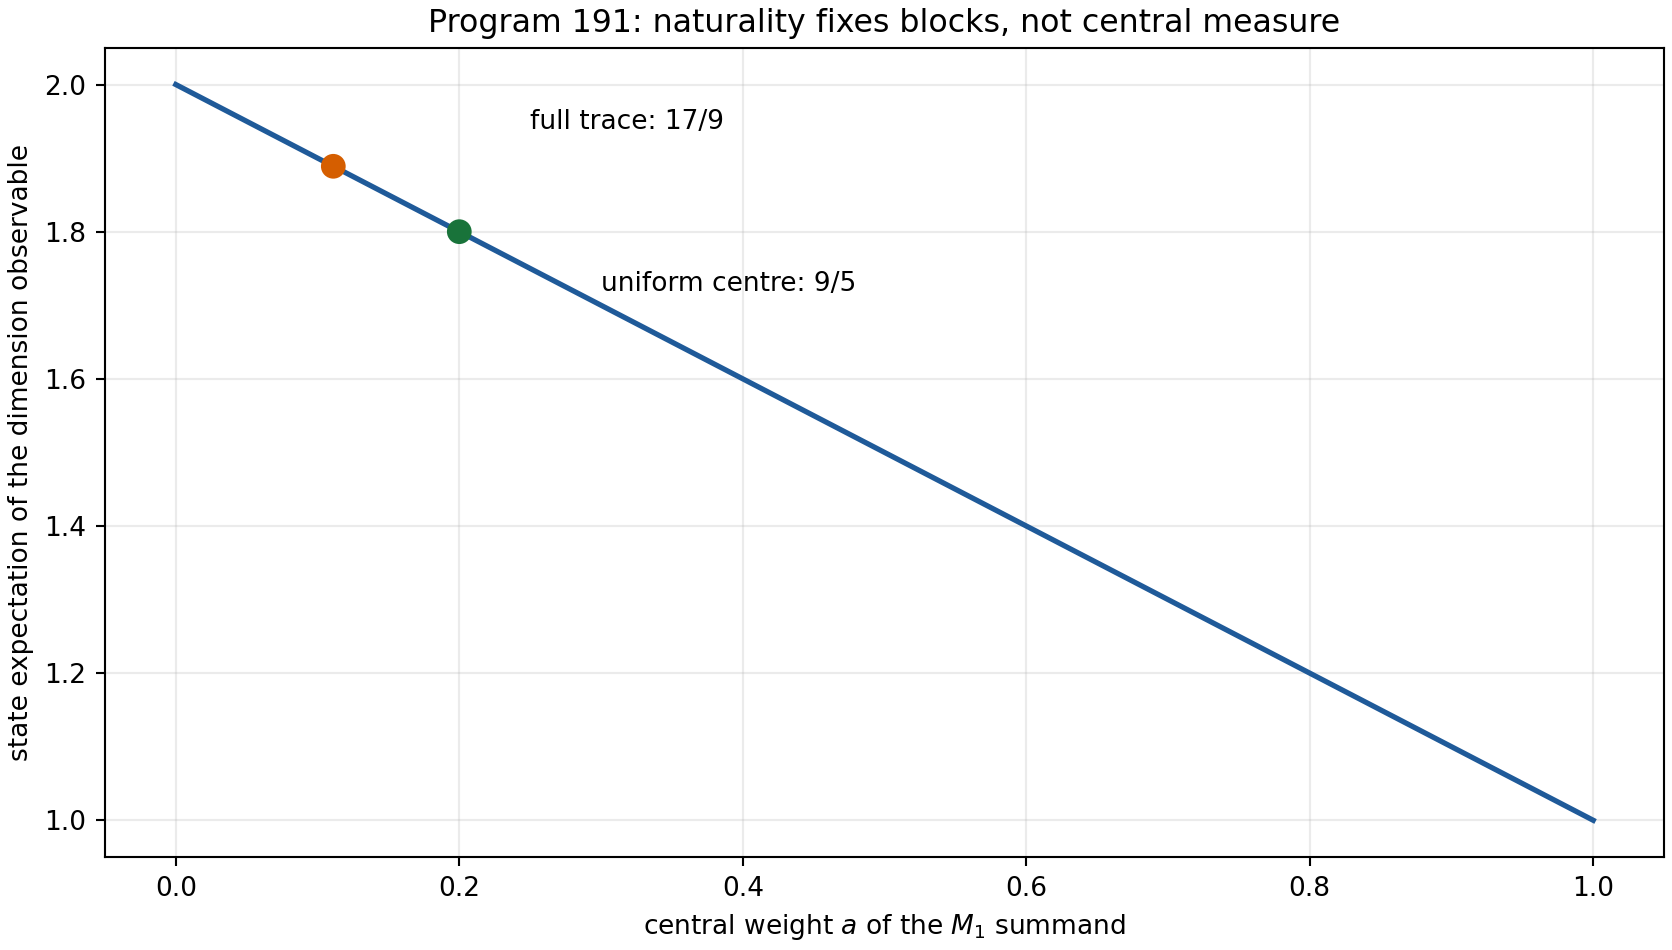
\includegraphics[width=0.94\textwidth]{FIN_Programs_191_203_Reference_Process_Prediction_Figures/program191_reference_state_naturality.png}
\caption{Inner-unitary naturality fixes normalized trace within blocks but leaves a central probability measure.}
\end{figure}

\section{Verdict}

\textbf{Proven.} Normalized trace is unique on each simple block, not on the non-simple algebra. A central measure, or a stronger principle such as a specified Morita-natural trace convention, is the exact missing datum. Neither \(9/5\) nor \(17/9\) is promoted to a strict state or temperature source.

\par\medskip\hrule\medskip

\chapter{Program 192 --- Beta-gauge invariant bridge observables}

\section{Scale action}

Under a change of length coordinate

\[
d'=cd,
\qquad c>0,
\]

the kernel family preserves its functional form if

\[
\beta'=\beta c^{-\eta},
\qquad
\omega'=\frac{\omega}{c},
\qquad
\eta'=\eta,
\qquad
\phi'=\phi.
\]

The positive \(\beta\) values form a torsor for this action.

\section{Quotient theorem}

Define

\[
x=\beta^{1/\eta}d,
\qquad
\nu=\frac{\omega}{\beta^{1/\eta}}.
\]

Then the amplitude-normalized kernel becomes

\[
\widehat K(x)
=
\frac{\cos(\nu x+\phi)}
{1+x^\eta}.
\]

Both \(x\) and \(\nu\) are invariant under the scale action. Thus \((\eta,\nu,\phi)\) and the reduced profile are genuine quotient data.

The numerical orbit audit spans \(c\in[10^{-4},10^4]\) and gives maximum profile residual

\[
1.11\times10^{-16}.
\]

\section{Legacy versus strict after quotient}

The invariant tuples are

\[
(\eta_\ell,\nu_\ell,\phi_\ell)
=
\left(
1,
\frac{\pi/4}{0.01},
\frac{\pi}{6}
\right)
=
(1,78.539816\ldots,0.523598\ldots)
\]

and

\[
(\eta_s,\nu_s,\phi_s)
=(1.8,0.18575,0.1625).
\]

Their reduced-profile RMS separation on \(x\in[0,8]\) is

\[
0.3816158693.
\]

\begin{figure}[htbp]
\centering
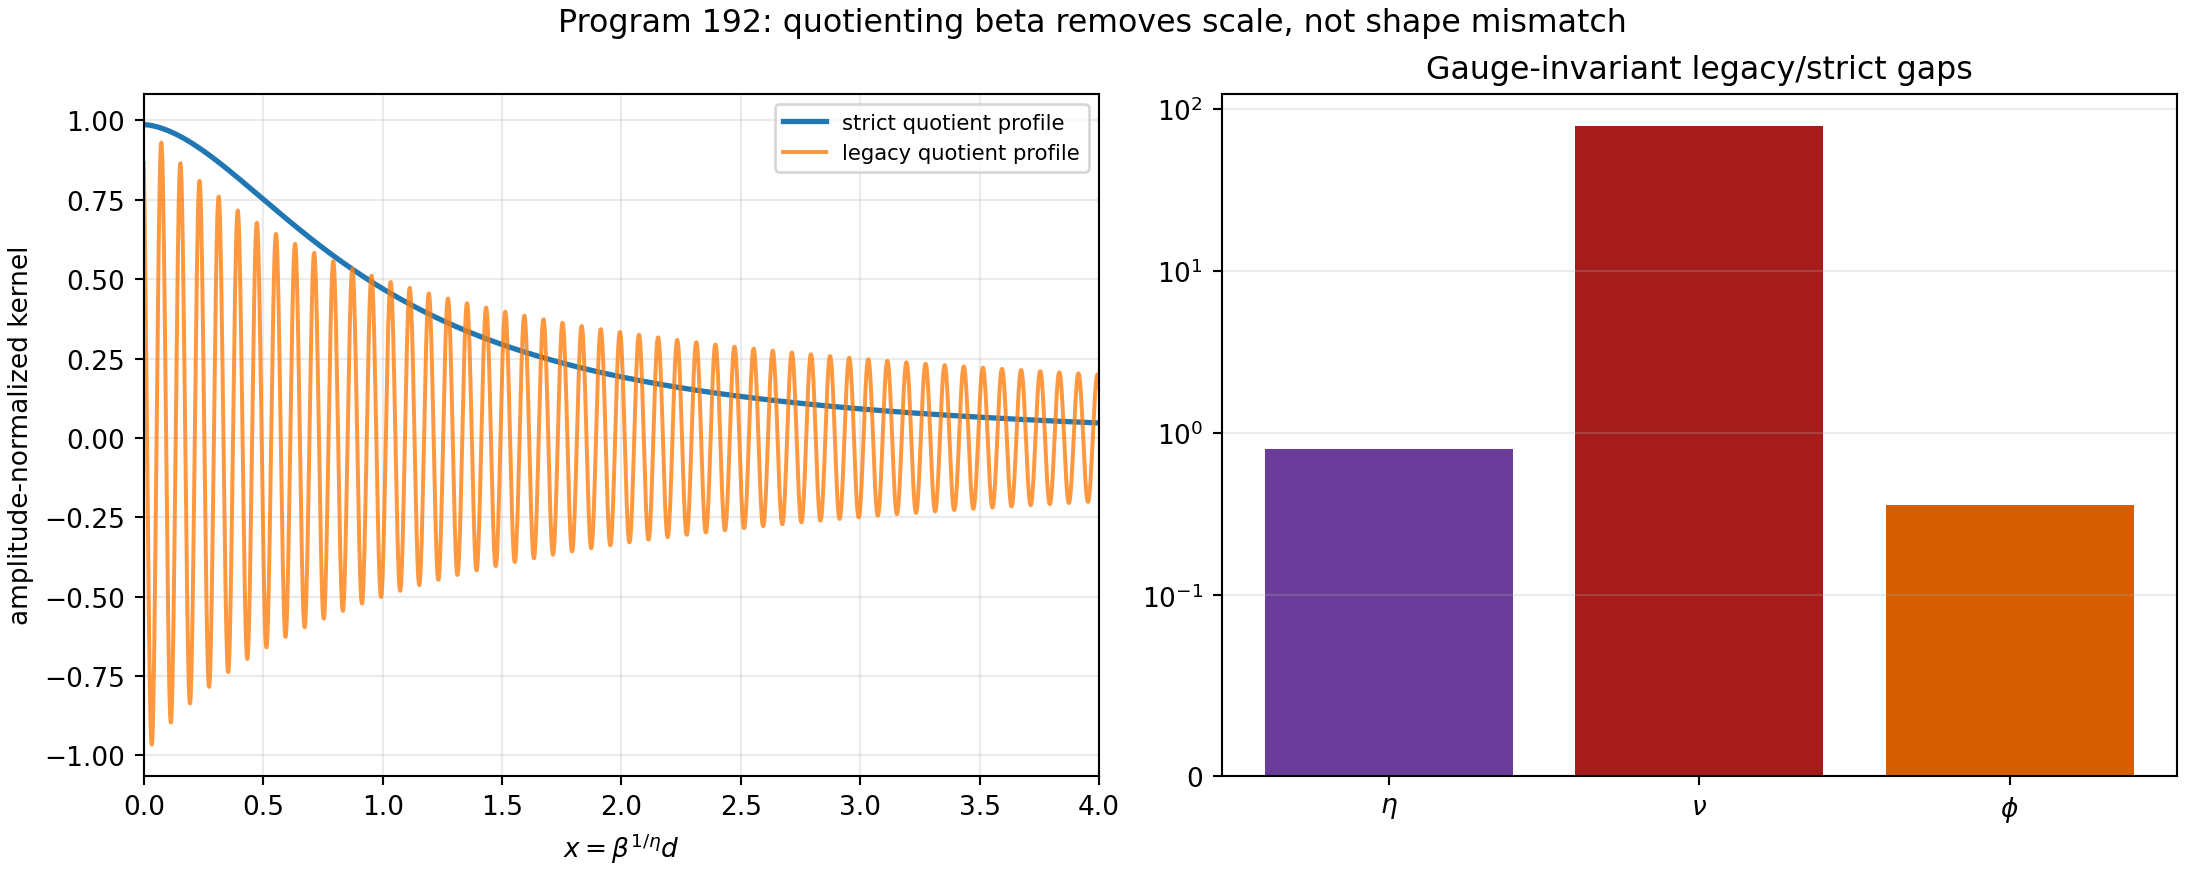
\includegraphics[width=0.94\textwidth]{FIN_Programs_191_203_Reference_Process_Prediction_Figures/program192_beta_gauge_quotient.png}
\caption{Quotienting the positive \(\beta\) torsor removes coordinate scale while preserving the strict--legacy shape mismatch.}
\end{figure}

\section{Verdict}

\textbf{Proven.} Setting \(\beta=1\) is a legitimate working gauge within a fixed positive orbit. It is not a strict source theorem. More importantly, removing the coordinate scale does not remove the invariant exponent, frequency, and phase differences. The legacy-to-strict bridge remains open, and no physical role transfer is licensed.

\par\medskip\hrule\medskip

\chapter{Program 193 --- Common-engine Arb certificate}

\section{Acceptance rule}

The desired fractional-symbol result requires five components in one directed-rounding engine:

\begin{enumerate}
\item 
finite FFT cells;

\item 
the average/\allowbreak{}polylogarithmic term;

\item 
the cancellation-correction tail;

\item 
denominator replacement;

\item 
resonant fallback modes.

\end{enumerate}

A formal sub-three-percent conclusion is admissible only if all five are enclosed in a common Arb or python-flint computation.

\section{Environment audit}

The local environment has neither an importable flint module nor an arb binary. Of the five components, one is already closed in the inherited certificate chain. The best inherited formal worst relative enclosure is

\[
0.6129831478,
\]

while the preregistered target is

\[
0.03.
\]

The analytic cancellation correction remains small:

\[
4.129713895\times10^{-7},
\]

but a small correction does not close the other interval obligations.

\begin{figure}[htbp]
\centering
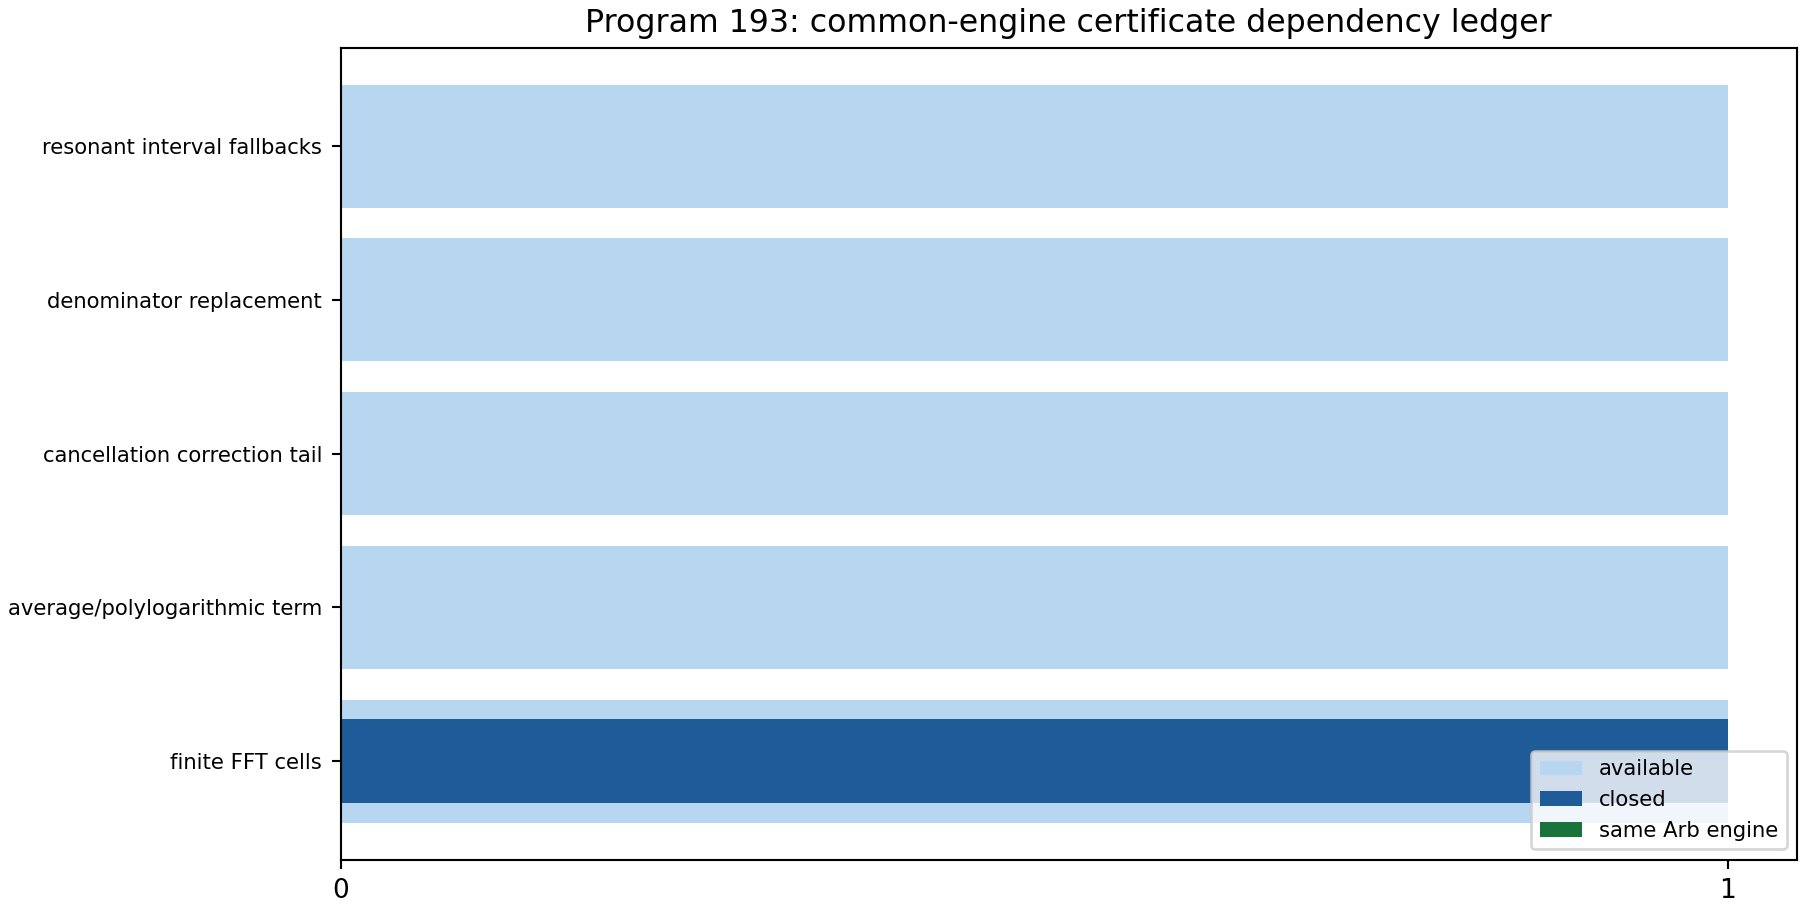
\includegraphics[width=0.94\textwidth]{FIN_Programs_191_203_Reference_Process_Prediction_Figures/program193_common_engine_certificate.png}
\caption{The common directed-rounding certificate remains blocked by missing engine closure for four components.}
\end{figure}

\section{Verdict}

\textbf{Open, with a proven dependency audit.} No common-engine formal certificate is claimed. The existing wide enclosure is an upper bound on uncertainty, not a formal lower bound on what a better engine could achieve. Therefore this program establishes a reproducible blocker rather than a mathematical impossibility.

\par\medskip\hrule\medskip

\chapter{Program 194 --- Compiled finite Dirichlet library}

\section{General theorem}

For finite symmetric \(W\ge0\) with row sum \(s\) and \(A=sI-W\):

\[
\begin{aligned}
\langle f,Af\rangle
&=
s\sum_x|f_x|^2
-\sum_{x,y}W_{xy}\overline{f_x}f_y \\
&=
\frac12\sum_{x,y}W_{xy}|f_x-f_y|^2
\ge0.
\end{aligned}
\]

Also

\[
A\mathbf1=0.
\]

Self-adjointness gives

\[
e^{-itA}{}^\ast e^{-itA}=I.
\]

For the heat semigroup,

\[
e^{-tA}
=
e^{-st}e^{tW}.
\]

Because every coefficient in the series for \(e^{tW}\) is entrywise nonnegative, the heat matrix is entrywise nonnegative. Since \(A\mathbf1=0\),

\[
e^{-tA}\mathbf1=\mathbf1.
\]

Thus it is stochastic in the declared finite graph convention.

\section{Executed checks}

The release checks 150 exact rational test vectors on cycle graphs with \(3\le n\le12\). Every exact quadratic form equals its Dirichlet sum and is nonnegative.

For the twelve-cycle numerical semigroups:

\begin{itemize}
\item 
maximum unitary residual: below \(10^{-13}\);

\item 
maximum heat row-sum residual: below \(10^{-13}\);

\item 
minimum heat entry: nonnegative up to floating-point noise.

\end{itemize}

\begin{figure}[htbp]
\centering
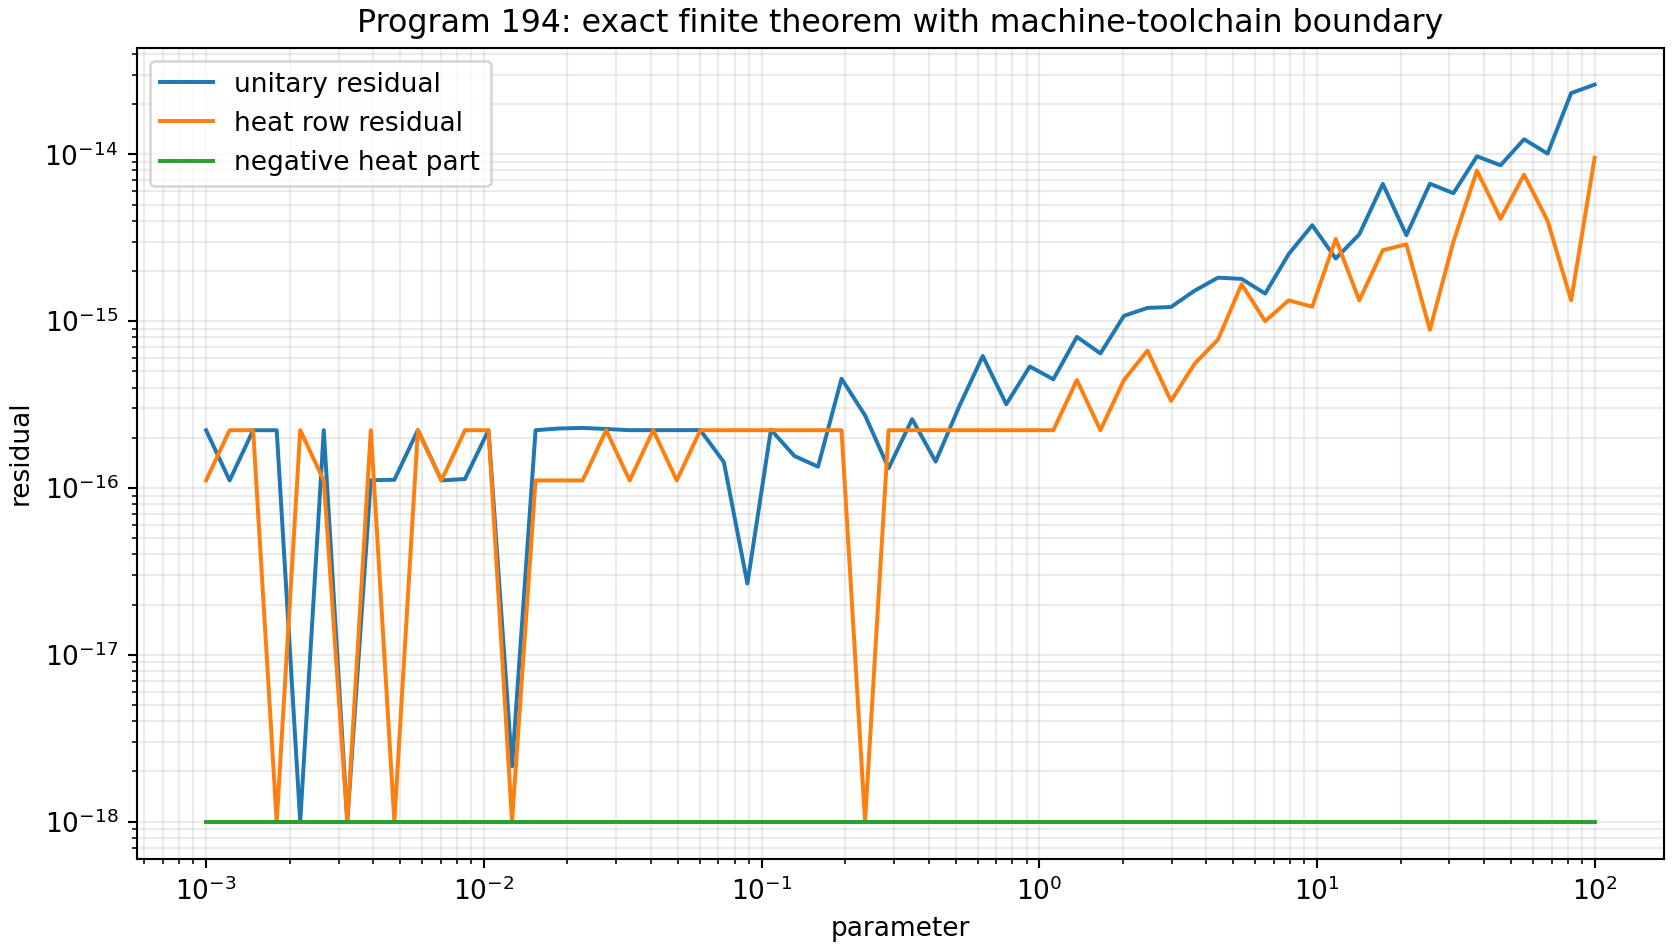
\includegraphics[width=0.94\textwidth]{FIN_Programs_191_203_Reference_Process_Prediction_Figures/program194_dirichlet_library.png}
\caption{Exact finite Dirichlet mathematics and numerical semigroup residuals, with proof-assistant compilation kept separate.}
\end{figure}

\section{Formal-tool boundary}

A general Lean source file is supplied. The local lean command is only an Elan launcher and no installed Lean toolchain is present. The source was not machine compiled. This report therefore distinguishes:

\begin{itemize}
\item 
the paper proof: \textbf{Proven};

\item 
exact rational executions: \textbf{Proven, computer-assisted};

\item 
proof-assistant compilation: \textbf{Open}.

\end{itemize}

No continuum limit, Born rule, apparatus, or physical interpretation follows from the finite theorem alone.

\par\medskip\hrule\medskip

\chapter{Program 195 --- Analytic reflection-conversion geometry}

\section{State and symmetry}

Consider real-plane qubit states

\[
\rho(r,z)
=
\frac12(I+r\sigma_x+z\sigma_z),
\qquad
r^2+z^2\le1,
\]

and the reflection \(R=\sigma_z\), which maps \(r\mapsto-r\).

A reflection-covariant channel mapping \(\rho_s\) to \(\rho_t\) exists if and only if a channel maps the ordered pair

\[
(\rho_s,R\rho_sR)
\quad\text{to}\quad
(\rho_t,R\rho_tR).
\]

The nontrivial direction follows by twirling a pair-mapping channel over \(\mathbb Z_2\).

\section{Alberti--Uhlmann reduction}

For qubits, the two-state transformation exists exactly when

\[
\|\rho_s-qR\rho_sR\|_1
\ge
\|\rho_t-qR\rho_tR\|_1
\quad
\text{for all }q\ge0.
\]

Direct diagonalization gives

\[
\|\rho-qR\rho R\|_1
=
\max\left\{
|1-q|,
\sqrt{(1+q)^2r^2+(1-q)^2z^2}
\right\}.
\]

Divide by \(1+q\) and set

\[
u=\frac{|1-q|}{1+q}\in[0,1].
\]

Define

\[
g_{r,z}(u)
=
\max\left\{
u,\sqrt{r^2+u^2z^2}
\right\}.
\]

The complete criterion is

\[
g_{r_s,z_s}(u)
\ge
g_{r_t,z_t}(u)
\qquad
\forall u\in[0,1].
\]

\section{Closed boundary}

For fixed \(z_t\), the largest reachable transverse coordinate satisfies

\[
r_{t,\max}^2
=
\min_{0\le x\le1}
\left[
\max\{x,r_s^2+xz_s^2\}
-xz_t^2
\right],
\qquad x=u^2.
\]

The expression is convex and piecewise linear in \(x\). Its minimum occurs at an endpoint or at the unique source kink

\[
x_c=\frac{r_s^2}{1-z_s^2}.
\]

Therefore

\[
r_{t,\max}^2
=
\min_{x\in\{0,1,x_c\}}
\left[
\max\{x,r_s^2+xz_s^2\}
-xz_t^2
\right].
\]

This removes numerical optimization completely.

\section{Falsification and cross-check}

For the source \((r_s,z_s)=(0.6,0)\) and target \(z_t=0.8\):

\[
x_c=0.36
\]

and

\[
r_{t,\max}^2
=
0.1296,
\qquad
r_{t,\max}=0.36.
\]

Thus the target \((0.6,0.8)\) is outside the conversion cone even though it passes the earlier scalar \(M\) comparison.

Five hundred random physical-state tests compare the closed formula against the previous dense Choi optimization. The maximum discrepancy is

\[
6.68\times10^{-6},
\]

consistent with the grid resolution of the older method.

\begin{figure}[htbp]
\centering
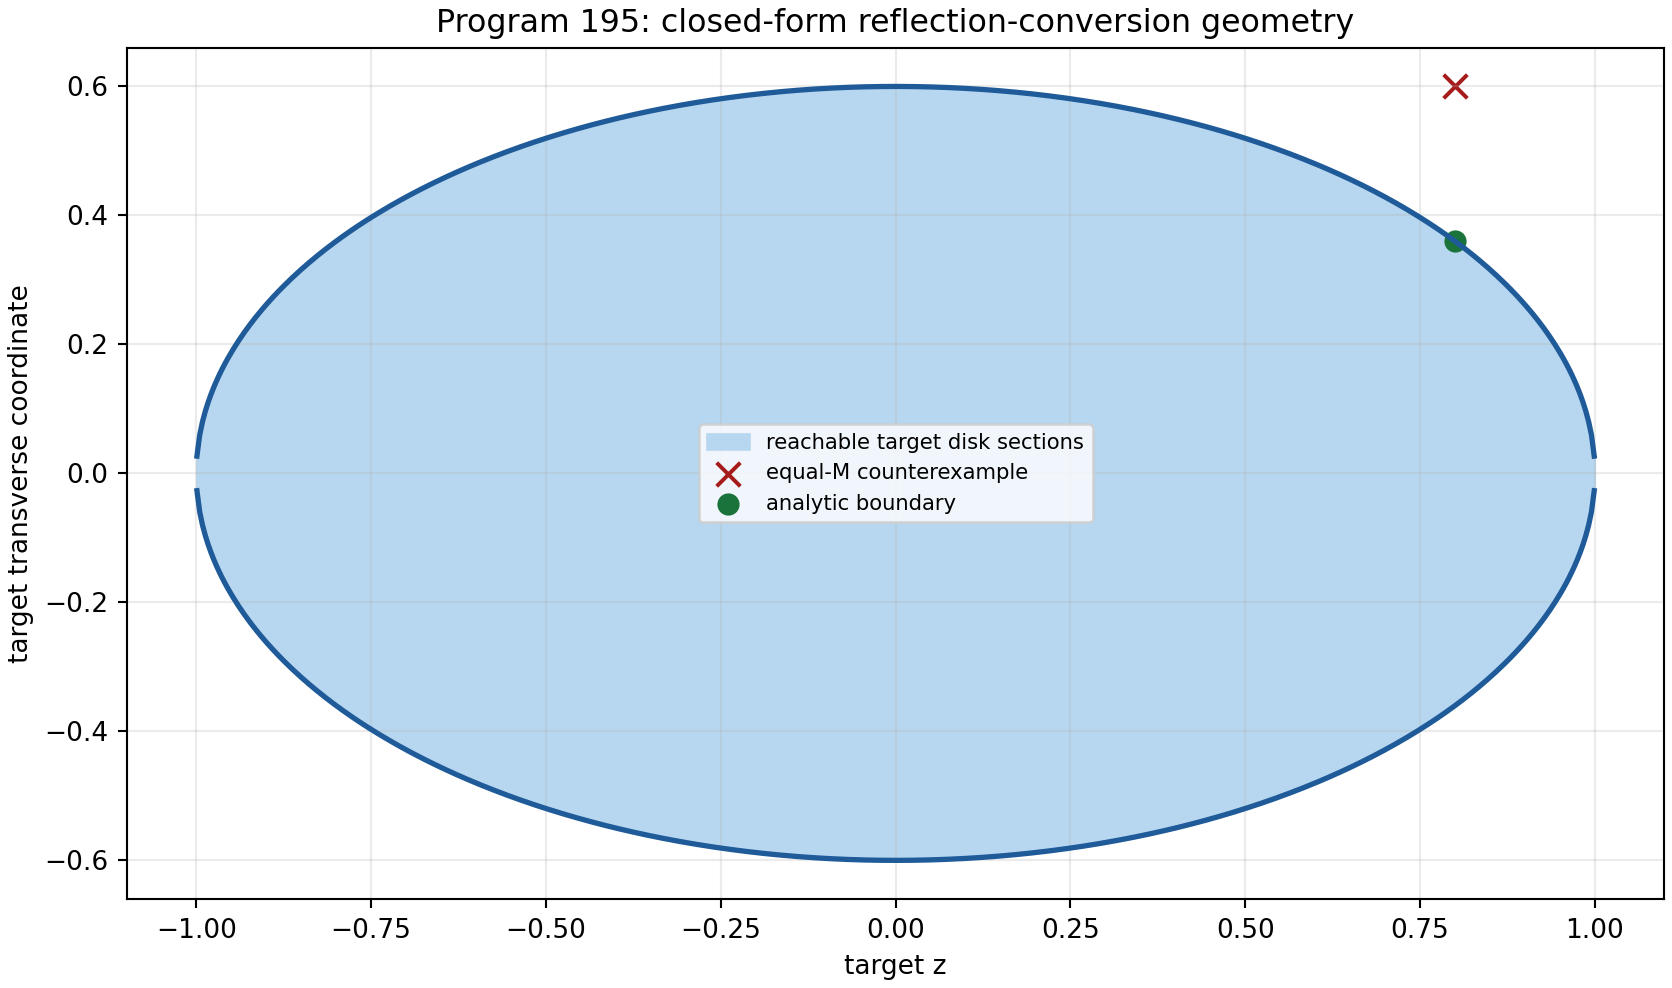
\includegraphics[width=0.94\textwidth]{FIN_Programs_191_203_Reference_Process_Prediction_Figures/program195_reflection_geometry.png}
\caption{Closed analytic reachability boundary for reflection-covariant conversion from the source state with transverse coordinate 0.6.}
\end{figure}

\section{Verdict}

\textbf{Proven.} The one-copy qubit reflection preorder is analytically complete in the declared setting. Tensor products leave the two-state qubit theorem; catalysis is not classified. The theorem consumes a supplied asymmetry resource. It does not create a signed preparation and does not discharge QW-2191.

\par\medskip\hrule\medskip

\chapter{Program 196 --- Mixing-aware empirical process theorem}

\section{Acquisition class}

Define an observed-refresh Markov chain. Let \(X_1\sim F\). For \(i\ge2\):

\begin{itemize}
\item 
with probability \(p\), draw a fresh independent value from \(F\);

\item 
with probability \(1-p\), repeat \(X_{i-1}\).

\end{itemize}

The acquisition system records every refresh flag. Its beta-mixing coefficient satisfies

\[
\beta(k)\le(1-p)^k.
\]

\section{Regenerative DKW theorem}

Let \(R\) be the number of recorded refresh blocks and keep the first value of each block. Conditional on \(R\), the retained variables are iid from \(F\). Therefore

\[
\Pr\left(
\sup_x|\widehat F_R(x)-F(x)|
>
\sqrt{\frac{\log(2/\delta)}{2R}}
\;\middle|\;R
\right)
\le\delta.
\]

Taking expectation over \(R\) preserves the same failure bound.

This theorem is nonasymptotic. The effective sample size is observed rather than guessed.

\section{Simulation}

The executed challenge uses:

\[
n=4000,
\qquad
p=0.05,
\qquad
\alpha=0.8,
\qquad
T=1/\alpha=1.25.
\]

Across 320 replicates:

\begin{itemize}
\item 
mean retained fraction: \(0.05029\);

\item 
invalid nominal-record coverage: \(0.85625\);

\item 
regenerative coverage: \(1.00000\);

\item 
valid intervals are substantially wider.

\end{itemize}

\begin{figure}[htbp]
\centering
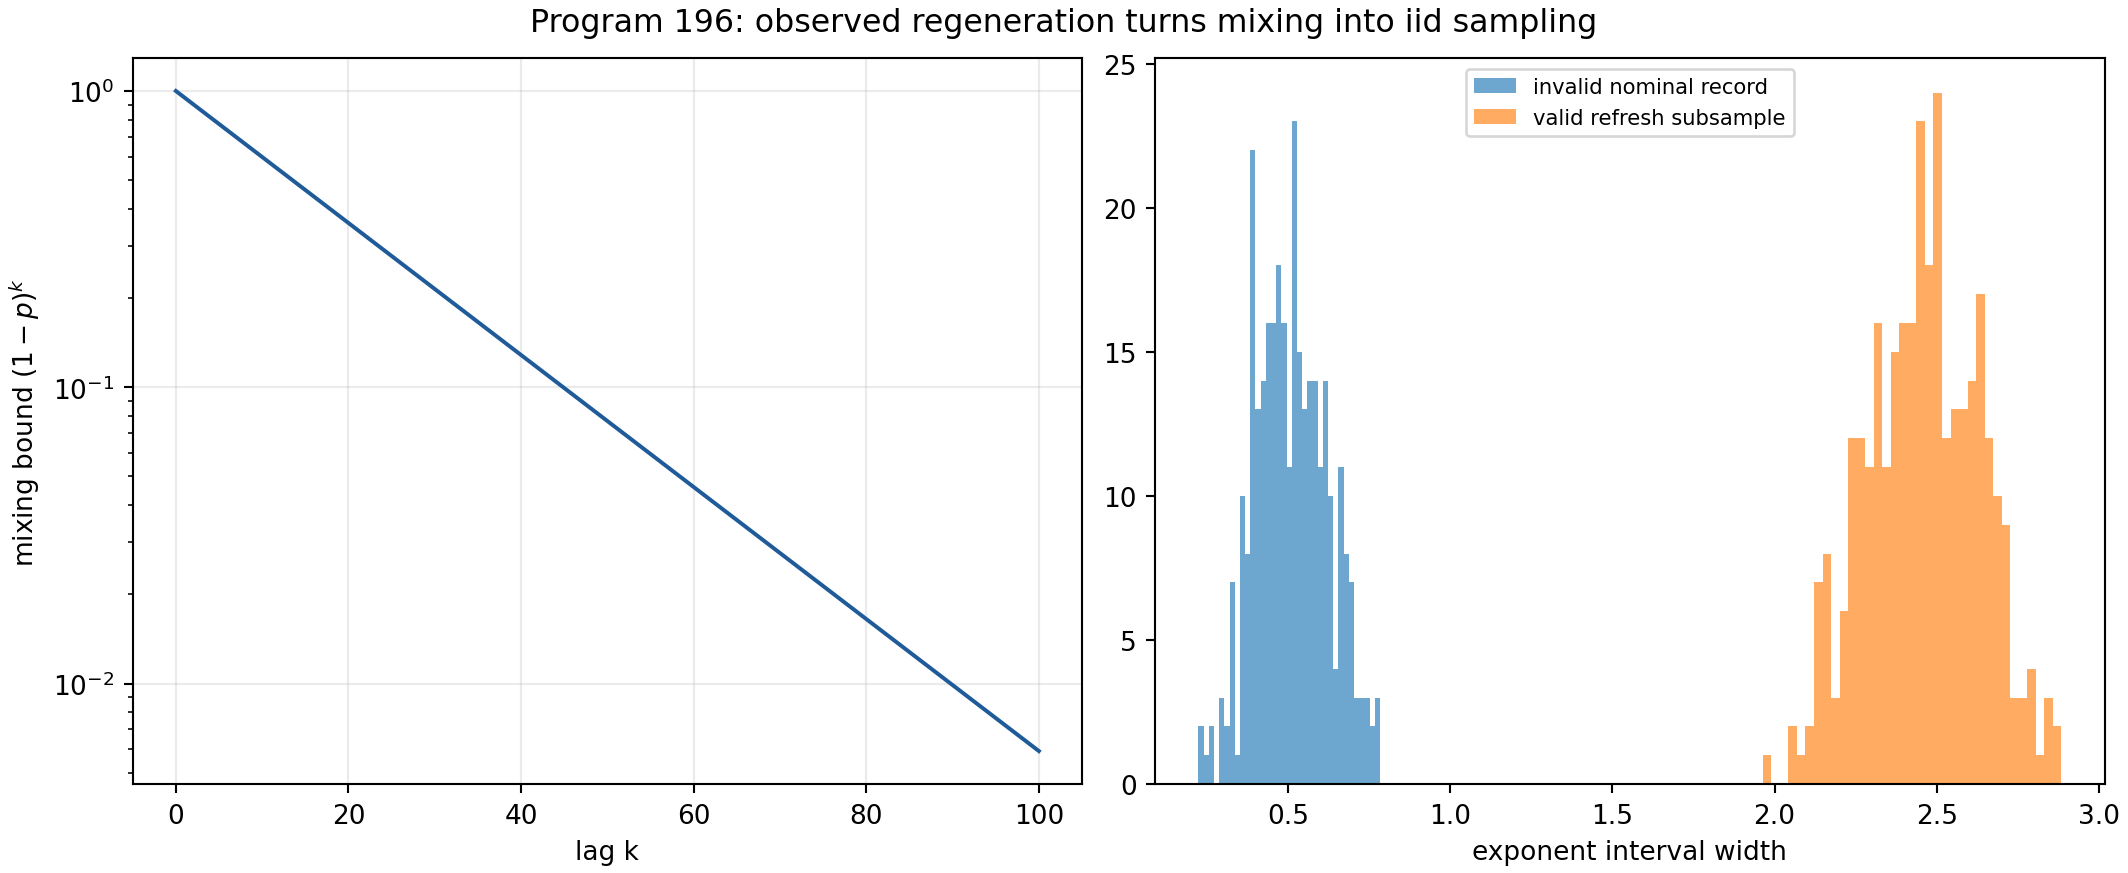
\includegraphics[width=0.94\textwidth]{FIN_Programs_191_203_Reference_Process_Prediction_Figures/program196_regenerative_mixing.png}
\caption{Observed regeneration supplies a valid iid subsample at a measurable information cost.}
\end{figure}

\section{Verdict}

\textbf{Proven for the declared acquisition class; strong numerical evidence for coverage.} The result does not solve arbitrary hidden beta mixing. Recorded regeneration is a real apparatus/\allowbreak{}acquisition assumption and must remain in the protocol.

\par\medskip\hrule\medskip

\chapter{Program 197 --- Order-sensitive open-set protocol}

\section{Motivation}

Program 185 proved that marginal quantile features are exactly invariant under time reordering. They therefore cannot identify memory.

Program 197 freezes six order-sensitive features before challenge execution:

\begin{enumerate}
\item 
lag-one Spearman correlation;

\item 
persistence of consecutive increment signs;

\item 
normalized ordinal-pattern entropy;

\item 
exact tie fraction;

\item 
time-versus-rank trend;

\item 
ordinal reversal asymmetry.

\end{enumerate}

The calibration score is a regularized Mahalanobis distance. Its rejection threshold is the empirical 0.99 quantile of 1,400 iid Gaussian calibration records, each of length 360.

\section{Frozen challenge}

Four hundred twenty records are generated for each of:

\begin{itemize}
\item 
independent Gaussian validation;

\item 
independent symmetric stable \(\alpha=0.8\);

\item 
sorted records with exactly the same Gaussian multisets;

\item 
Gaussian AR(1) with coefficient \(0.8\);

\item 
exact repeated blocks of length 20;

\item 
Gaussian records with linear drift.

\end{itemize}

The sorted challenge preserves every one-time empirical multiset exactly:

\[
\max
\left|
\operatorname{sort}(x)
-
\operatorname{sort}(\operatorname{sort}(x))
\right|
=0.
\]

\section{Results}

\begin{center}
\begingroup\small
\setlength{\tabcolsep}{3.5pt}
\renewcommand{\arraystretch}{1.16}
\begin{longtable}{@{}p{0.420\textwidth}p{0.420\textwidth}@{}}
\toprule
\textbf{Challenge} & \textbf{Rejection rate} \\
\midrule
\endhead
iid Gaussian validation & 0.01429 \\
iid stable \(\alpha=0.8\) & 0.00714 \\
sorted same multiset & 1.00000 \\
AR(1), \(\phi=0.8\) & 1.00000 \\
repeated block 20 & 1.00000 \\
linear drift & 1.00000 \\
\bottomrule
\end{longtable}
\endgroup
\end{center}

\begin{figure}[htbp]
\centering
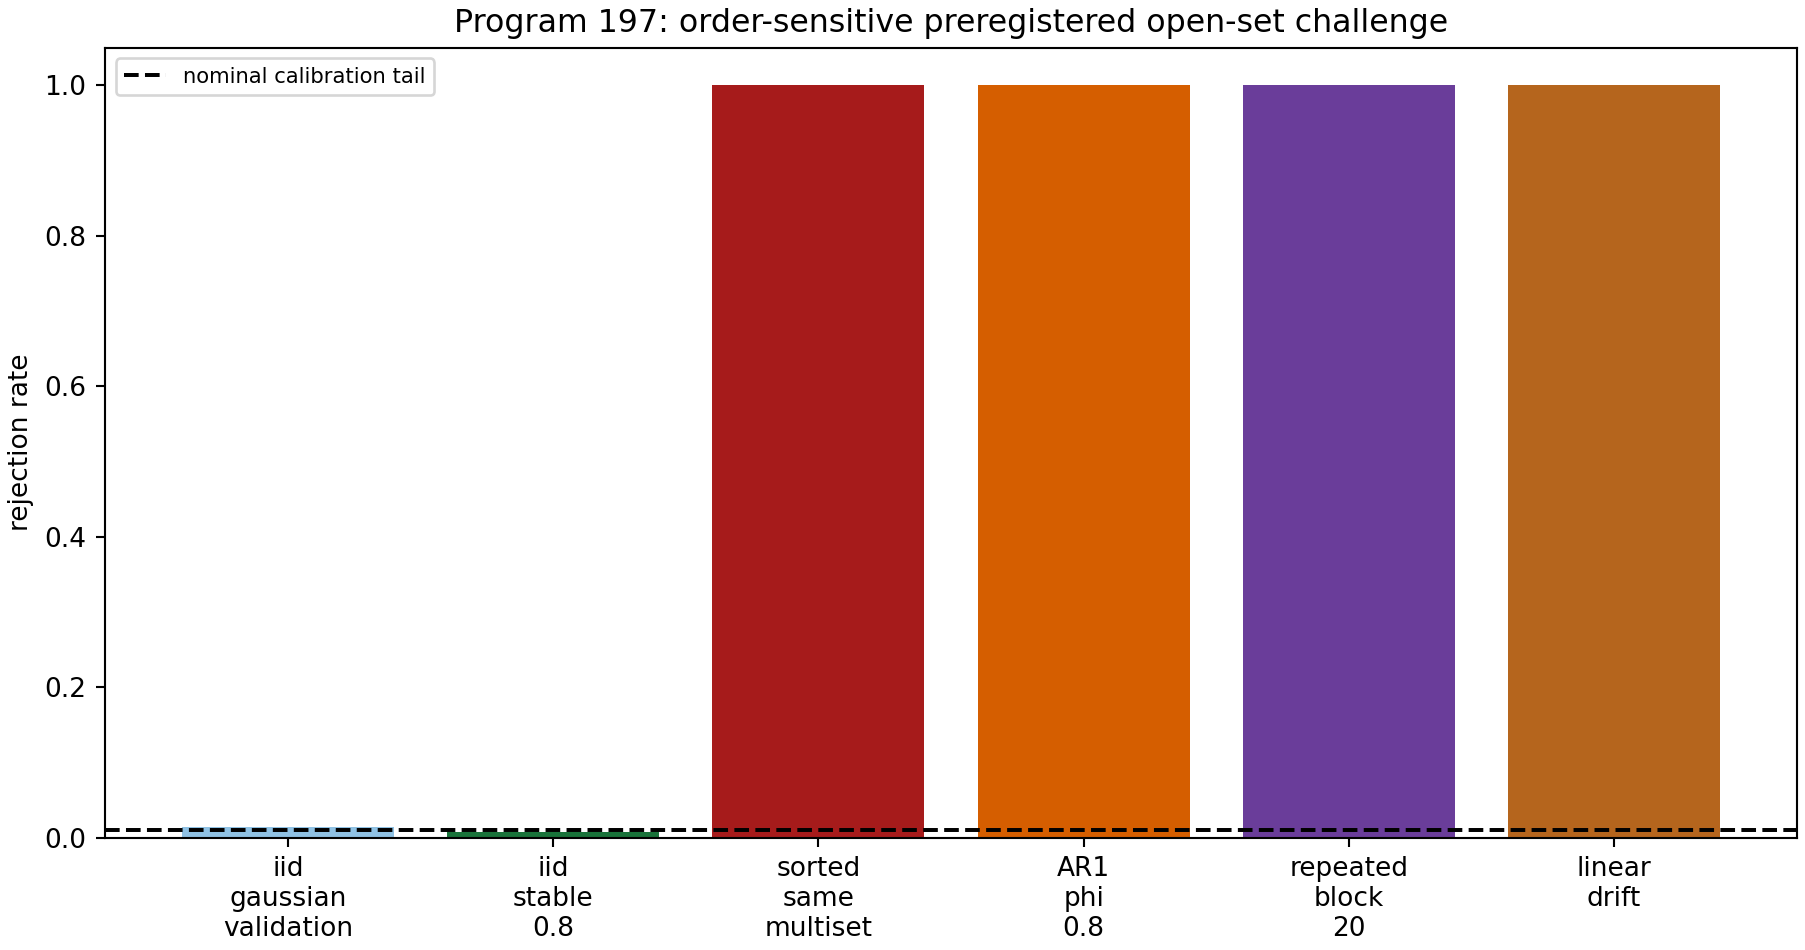
\includegraphics[width=0.94\textwidth]{FIN_Programs_191_203_Reference_Process_Prediction_Figures/program197_order_sensitive_open_set.png}
\caption{The frozen temporal feature protocol rejects four declared order-dependent alternatives while retaining iid specificity.}
\end{figure}

\section{Verdict}

\textbf{Strong synthetic evidence.} The protocol repairs the exact order blindness for the declared challenges and retains specificity under a continuous iid heavy-tailed law. It is not a universal open-set classifier, a proof that a record has one unique memory mechanism, or external validation.

\par\medskip\hrule\medskip

\chapter{Program 198 --- Minimal process-tensor tomography}

\section{Declared family}

Let two zero-mean Gaussian phase increments have common variance \(v\) and covariance \(c\). Let detector blur multiply every visibility by \(b\).

The three contrasts are:

\[
V_1=be^{-v/2},
\]

\[
V_+=be^{-(v+c)},
\]

\[
V_-=be^{-(v-c)}.
\]

\(V_-\) is the echo contrast.

\section{Rank theorem}

With

\[
\theta=
\begin{pmatrix}
\log b\\v\\c
\end{pmatrix},
\qquad
y=
\begin{pmatrix}
\log V_1\\
\log V_+\\
\log V_-
\end{pmatrix},
\]

the model is

\[
y=
\begin{pmatrix}
1&-1/2&0\\
1&-1&-1\\
1&-1&1
\end{pmatrix}
\theta.
\]

The matrix has determinant \(-1\) and rank three. Removing echo leaves two rows and rank two. In this three-parameter model, fewer than three scalar contrasts cannot be locally identifying.

The inverse is explicit:

\[
c
=
\frac12(\log V_--\log V_+),
\]

\[
v
=
2\log V_1-\log V_+-\log V_-,
\]

\[
\log b
=
2\log V_1
-\frac12(\log V_++\log V_-).
\]

\section{Noise challenge}

For truth

\[
b=0.84,
\qquad
v=0.45,
\qquad
c=0.20
\]

and Gaussian log-visibility noise of standard deviation \(0.015\), 6,000 replicates give mean parameter estimates within \(2\times10^{-4}\) of truth. The design condition number is \(7.2874\).

\begin{figure}[htbp]
\centering
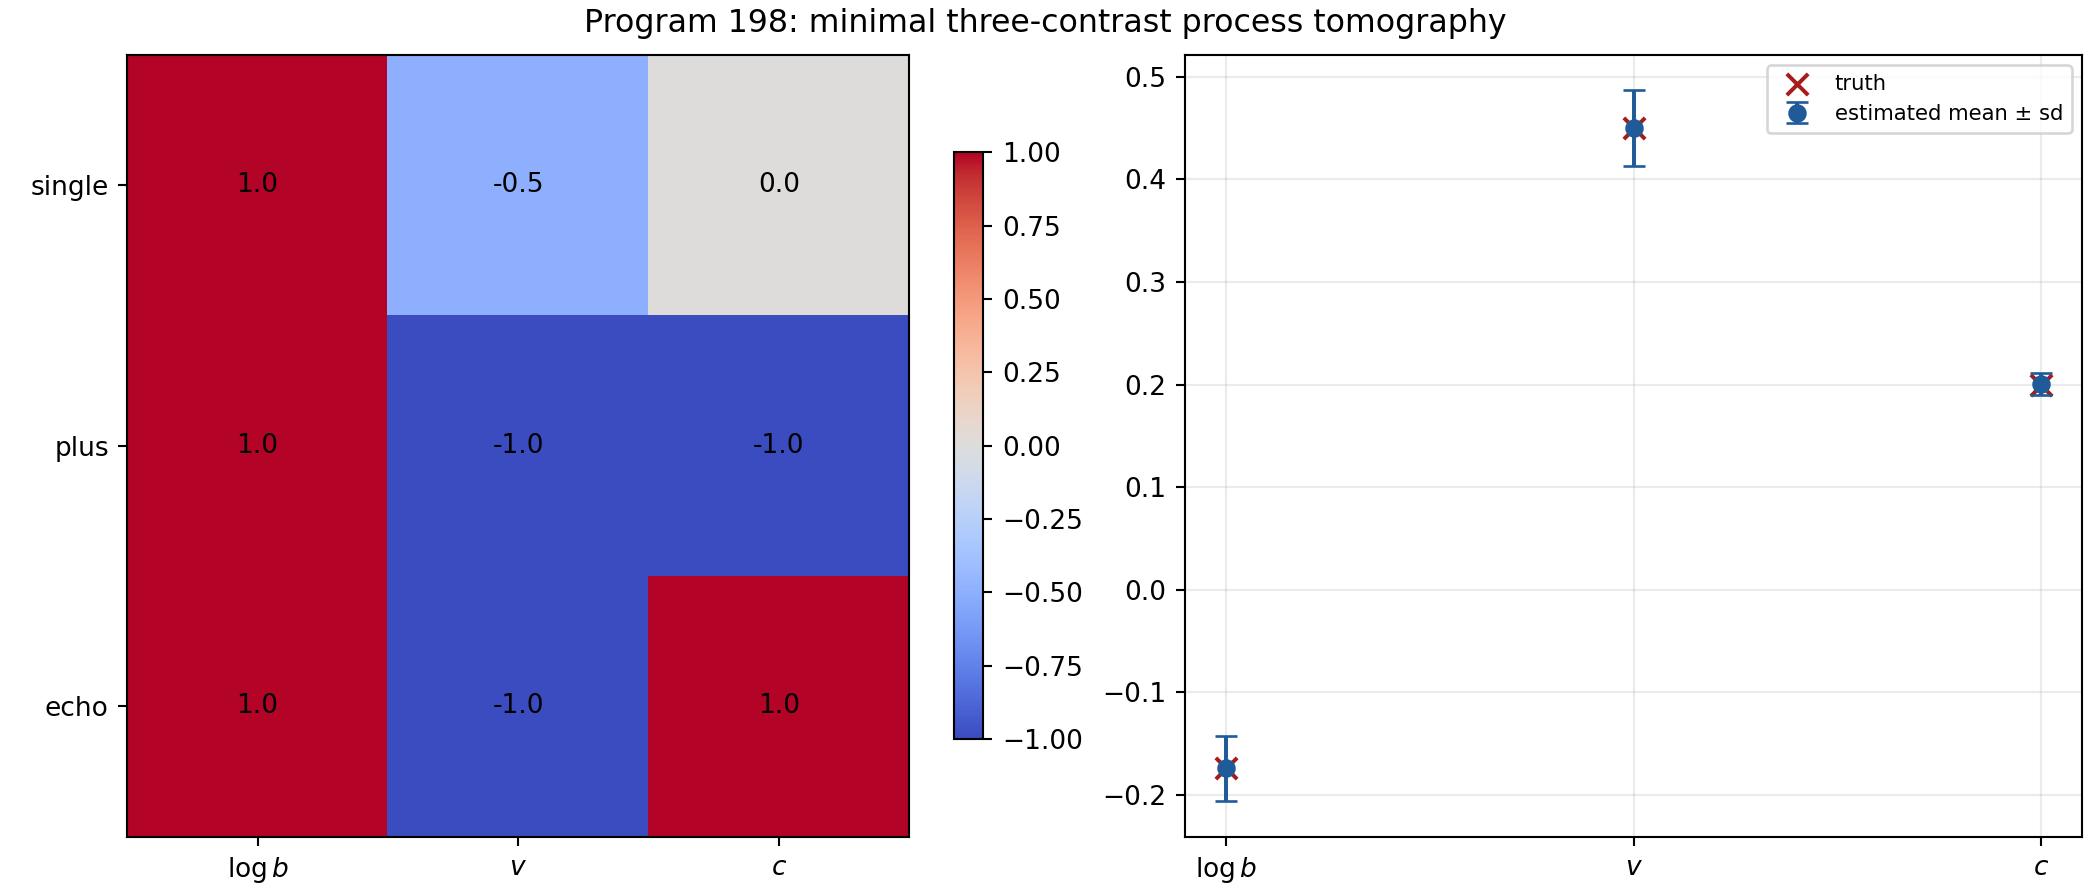
\includegraphics[width=0.94\textwidth]{FIN_Programs_191_203_Reference_Process_Prediction_Figures/program198_minimal_process_tomography.png}
\caption{The single, plus and echo log-visibility design has rank three and identifies blur, variance and covariance.}
\end{figure}

\section{Verdict}

\textbf{Proven in the declared Gaussian equal-variance family; strong finite-noise evidence.} Detector blur is separated as an explicit nuisance channel. Gaussianity, equal variance, and the visibility model are OP assumptions, not consequences of \(A\).

\par\medskip\hrule\medskip

\chapter{Program 199 --- Environment equivalence and causal identifiability}

\section{Operational quotient}

Define two environments to be \(k\)-equivalent when they yield the same probability for every preparation, intervention, and measurement in the declared \(k\)-step protocol.

The quotient class, rather than a microscopic dilation coordinate, is the operationally meaningful object.

Minimal Stinespring dilations of one channel are unique only up to an environment isometry. Nonminimal dilations have still larger redundancy.

\section{Explicit one-time counterexample}

Fix the one-step dephasing factor

\[
\gamma=0.8.
\]

Environment A has phase distribution

\[
\mu_A
=
\frac12\delta_{-a}
+\frac12\delta_a,
\qquad
a=\arccos(0.8).
\]

Environment B has

\[
\mu_B
=
0.9\delta_0+0.1\delta_\pi.
\]

Both have the same characteristic function at one:

\[
\widehat\mu_A(1)
=
\widehat\mu_B(1)
=0.8.
\]

Thus they produce the same one-time dephasing channel. At argument two:

\[
\widehat\mu_A(2)
=
\cos(2a)
=
2(0.8)^2-1
=0.28,
\]

while

\[
\widehat\mu_B(2)=1.
\]

They are distinguished by a suitable multi-time protocol.

\begin{figure}[htbp]
\centering
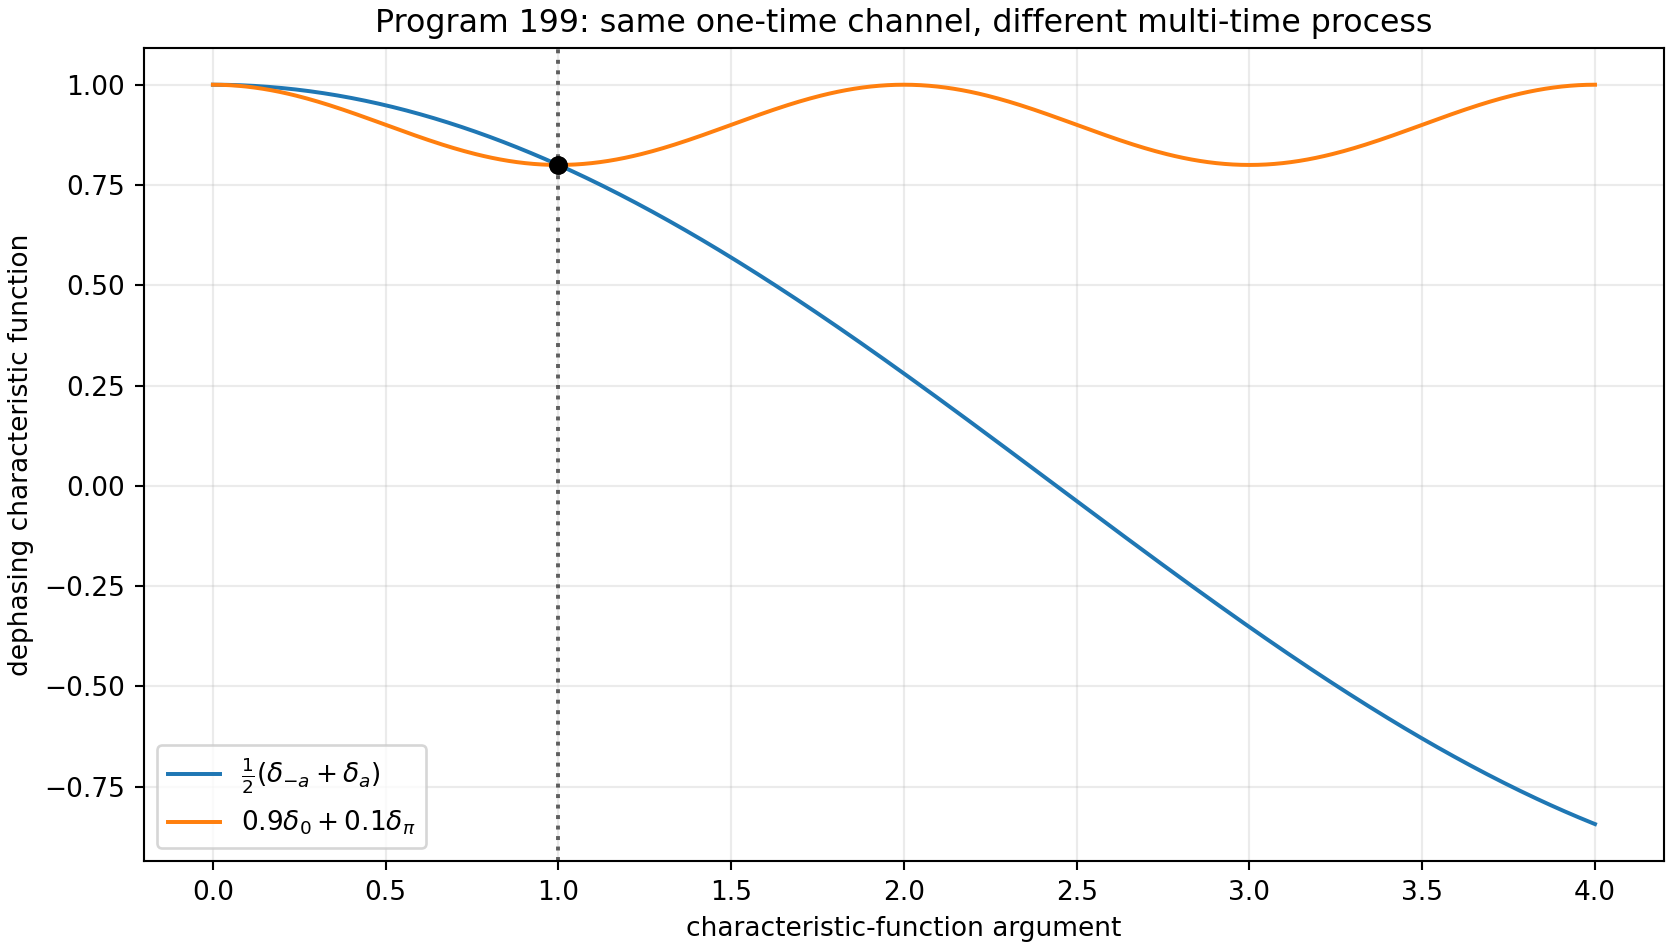
\includegraphics[width=0.94\textwidth]{FIN_Programs_191_203_Reference_Process_Prediction_Figures/program199_environment_equivalence.png}
\caption{Two distinct phase environments generate the same one-time dephasing channel but different two-time characteristics.}
\end{figure}

\section{Finite identifiability theorem}

A finite set of measured characteristic-function values is a finite-dimensional affine image of the infinite-dimensional probability measure simplex. Unless a finite parametric family is independently justified, its fibres generically contain multiple phase laws.

\section{Verdict}

\textbf{Proven by construction.} The microscopic environment is not determined by \(A\) or by one reduced channel. Process interventions refine the operational quotient but finite measurements do not identify an arbitrary environment distribution. Unidentifiable dilation coordinates cannot receive physical roles.

\par\medskip\hrule\medskip

\chapter{Program 200 --- Analytic phase-source classification}

\section{Source and target}

The legacy phase generator is

\[
z_\ell=e^{i\pi/4},
\]

an algebraic eighth root of unity. The strict frequency phase used in the audit is

\[
z_s=e^{i743/4000}.
\]

Since \(i743/4000\) is nonzero algebraic, Lindemann--Weierstrass implies that \(z_s\) is transcendental.

\section{Natural endomorphism no-go}

Every continuous group endomorphism

\[
f:U(1)\to U(1)
\]

has the form

\[
f(z)=z^n,
\qquad n\in\mathbb Z.
\]

Therefore \(f(z_\ell)\) is always a root of unity and can never equal \(z_s\). The closest value among the distinct order-eight endomorphism images remains at distance \(0.1854831\).

\section{Candidate audit}

\begin{center}
\begingroup\small
\setlength{\tabcolsep}{3.5pt}
\renewcommand{\arraystretch}{1.16}
\begin{longtable}{@{}p{0.261\textwidth}p{0.125\textwidth}p{0.262\textwidth}p{0.212\textwidth}@{}}
\toprule
\textbf{Operation class} & \textbf{Produces target?} & \textbf{Target-independent?} & \textbf{Verdict} \\
\midrule
\endhead
continuous \(U(1)\) endomorphism & no & yes & root-of-unity obstruction \\
algebraic functional calculus & no & yes & algebraicity obstruction \\
polynomial interpolation & yes & no & target inserted \\
logarithm and re-exponentiation & yes & no & branch and coefficient inserted \\
constant holomorphic map & yes & no & pure target coding \\
\bottomrule
\end{longtable}
\endgroup
\end{center}

\begin{figure}[htbp]
\centering
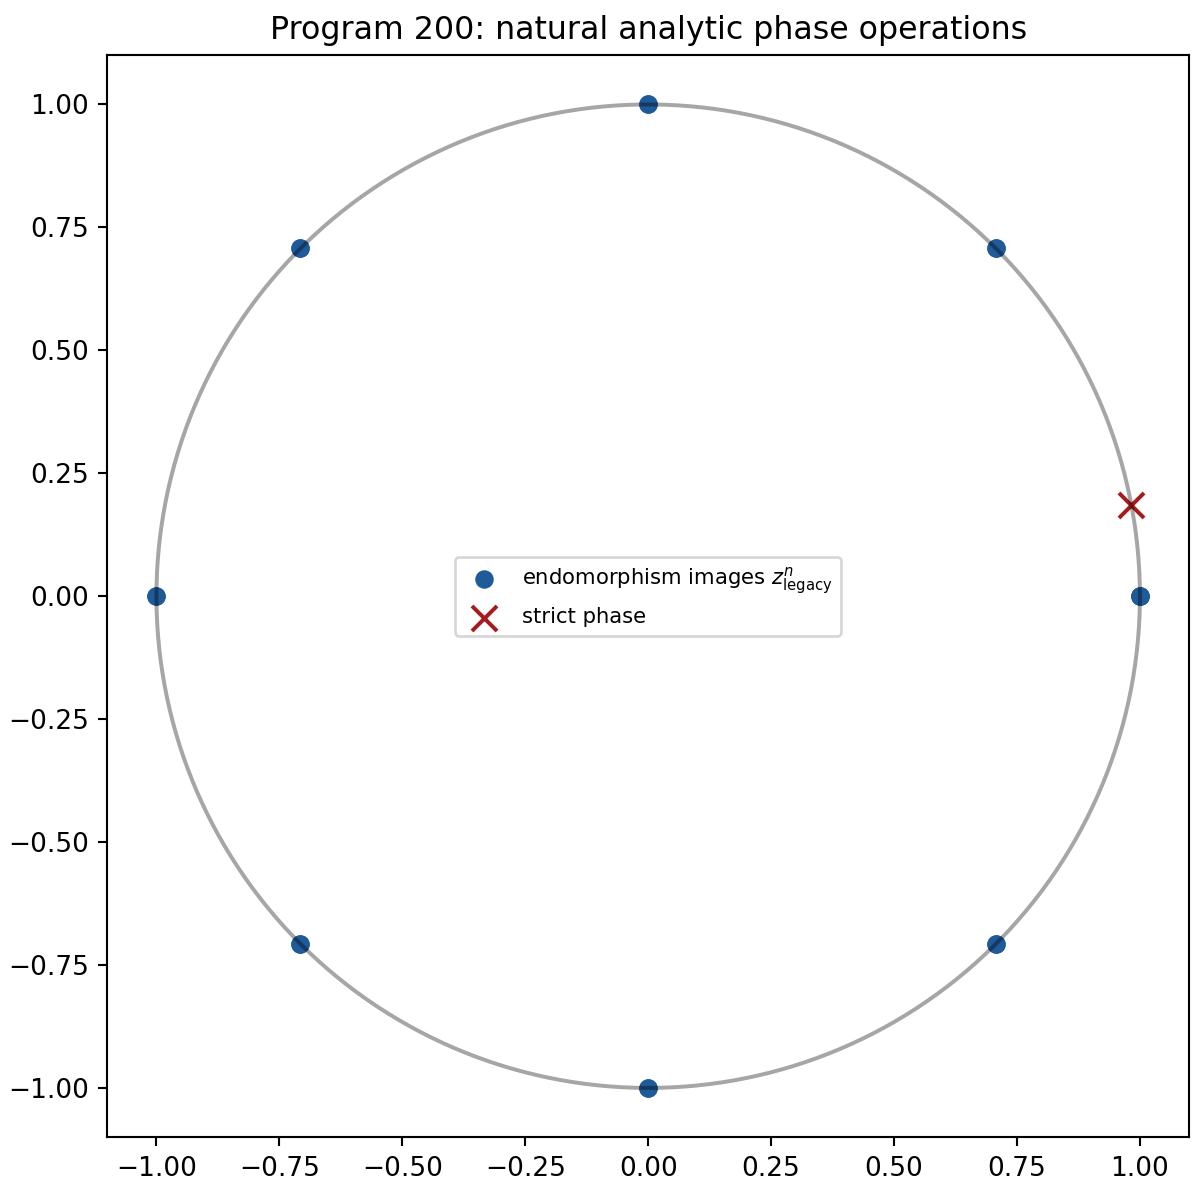
\includegraphics[width=0.94\textwidth]{FIN_Programs_191_203_Reference_Process_Prediction_Figures/program200_analytic_phase_sources.png}
\caption{Natural circle-group endomorphism images of the legacy phase miss the strict transcendental phase.}
\end{figure}

\section{Verdict}

\textbf{Proven for the declared operation classes.} Arbitrary analytic functions can interpolate a single source-target pair, so unconstrained analyticity has no provenance content. No accepted candidate supplies a repository-sourced origin, target-independent law, and coupling. The strict phase source remains open.

\par\medskip\hrule\medskip

\chapter{Program 201 --- Scale-free observable catalogue}

\section{Orbit}

The scale transformation is

\[
(A,t,z)\mapsto(cA,t/c,cz),
\qquad c>0.
\]

It preserves \(tA\) and transforms the resolvent covariantly:

\[
(cA+czI)^{-1}
=
\frac1c(A+zI)^{-1}.
\]

\section{Projective observable algebra}

Every invariant observable factors through the projective spectral class \([A]\) together with dimensionless combinations. Executable representatives include:

\begin{itemize}
\item 
eigenvalue ratios;

\item 
condition number on the positive support;

\item 
spectral probability entropy;

\item 
heat trace at fixed \(\tau=t\lambda_{\rm gap}\);

\item 
gap-normalized resolvent at fixed \(z/\lambda_{\rm gap}\);

\item 
unitary transition probabilities at fixed \(t\lambda_{\rm gap}\);

\item 
the beta-gauge quotient profile \((\eta,\nu,\phi)\).

\end{itemize}

Noninvariants include:

\begin{itemize}
\item 
the raw spectral gap;

\item 
raw time;

\item 
raw resolvent energy;

\item 
a raw positive \(\beta\) representative;

\item 
mass, length, and energy in physical units.

\end{itemize}

\section{Audit}

On the twelve-cycle, \(c\) spans \(10^{-6}\) through \(10^6\). The raw gap changes by

\[
10^{12}.
\]

The largest residual among the normalized spectrum, condition number, spectral entropy, dimensionless heat trace, and dimensionless resolvent is below

\[
8\times10^{-14}.
\]

\begin{figure}[htbp]
\centering
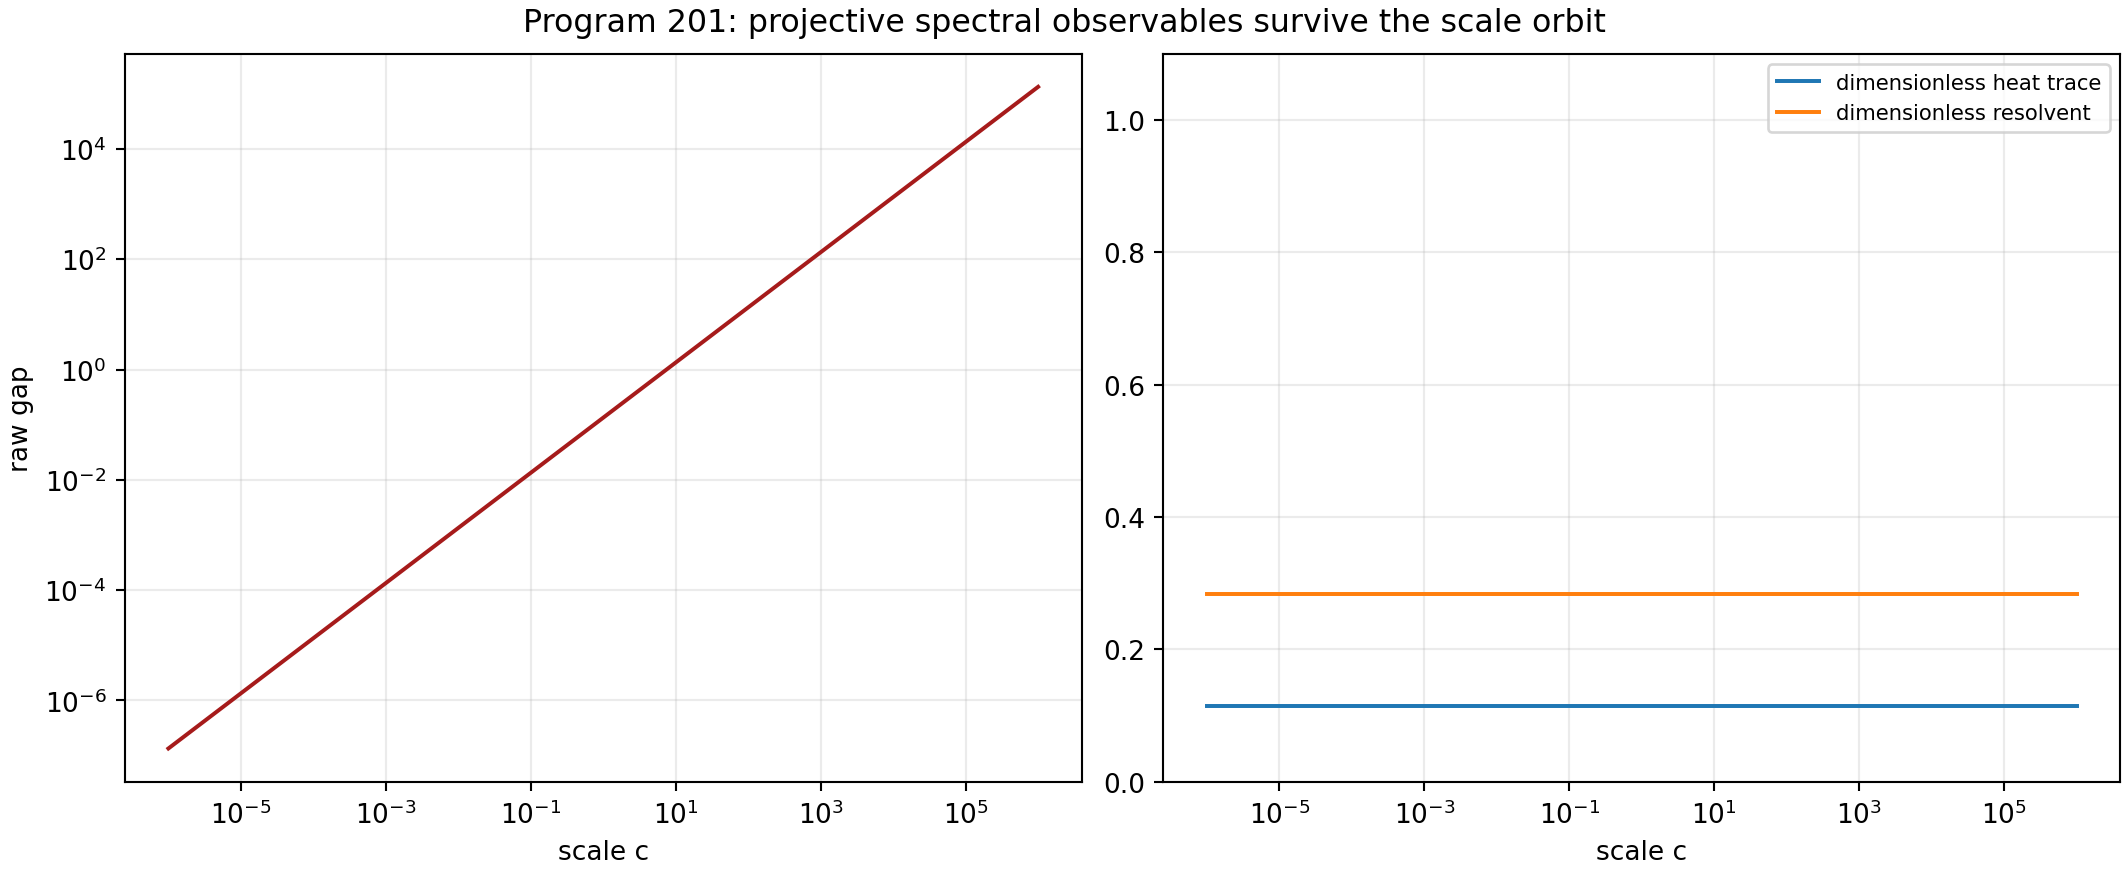
\includegraphics[width=0.94\textwidth]{FIN_Programs_191_203_Reference_Process_Prediction_Figures/program201_scale_free_observables.png}
\caption{The raw gap changes over twelve decades while projective heat and resolvent observables remain invariant.}
\end{figure}

\section{Verdict}

\textbf{Proven.} Before a physical clock or scale source is supplied, only projective/\allowbreak{}dimensionless observables are admissible for strict falsification. This does not make dimensionful quantities impossible; it shows exactly where CA or a new scale-charged strict source enters.

\par\medskip\hrule\medskip

\chapter{Program 202 --- Admissible experimental bundle}

\section{Intake fields}

The frozen gate requires:

\begin{enumerate}
\item 
public source identifier;

\item 
explicit license;

\item 
immutable hashes;

\item 
preparation provenance;

\item 
raw time-ordered records;

\item 
units and timestamps;

\item 
detector calibration;

\item 
apparatus-memory calibration;

\item 
reference control;

\item 
exclusion audit;

\item 
independent analysis boundary.

\end{enumerate}

\section{Constructed dry-run bundle}

An event-level synthetic bundle is generated with 12,000 ordered binary events. It contains five phase-scan contexts:

\begin{itemize}
\item 
reference;

\item 
single;

\item 
plus;

\item 
echo;

\item 
held-out.

\end{itemize}

It records sequence number, conditional seconds, context, intervention coefficients, phase in radians, and binary outcome. The data hash is frozen in the metadata.

Ten of eleven fields pass. The independent-analysis boundary fails because the generator and evaluator belong to the same release. The source class is explicitly

synthetic\_method\_validation.

\begin{figure}[htbp]
\centering
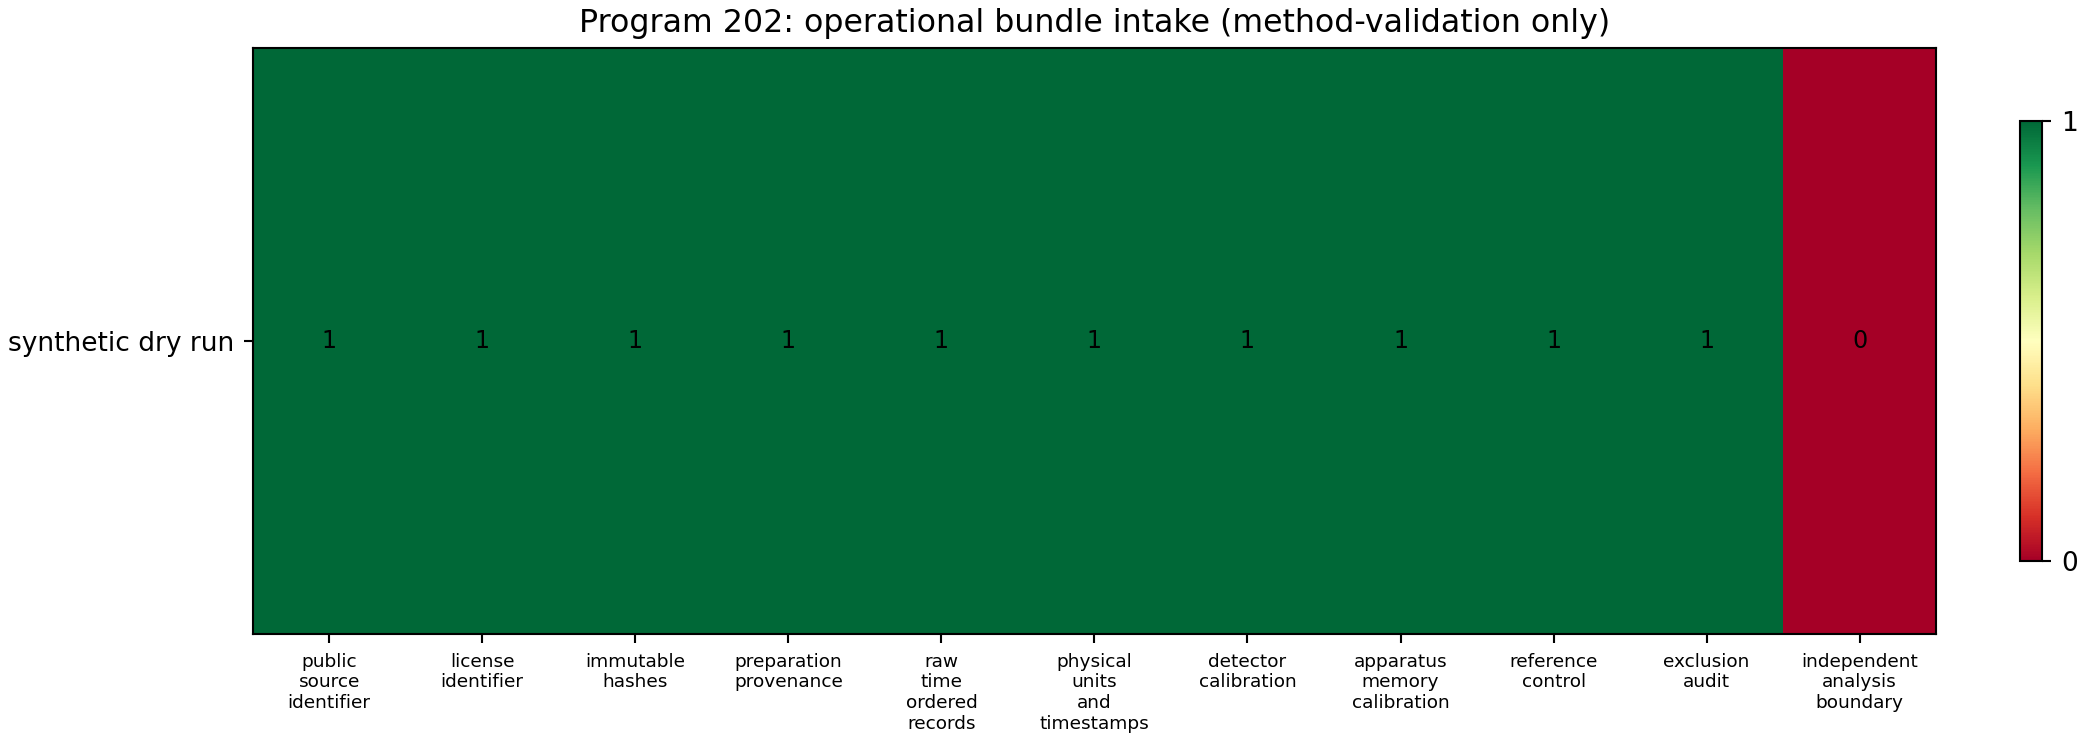
\includegraphics[width=0.94\textwidth]{FIN_Programs_191_203_Reference_Process_Prediction_Figures/program202_operational_bundle.png}
\caption{The synthetic method-validation bundle passes ten of eleven intake fields and fails independent provenance.}
\end{figure}

\section{Verdict}

\textbf{Proven schema and hash audit.} The bundle demonstrates that the operational gate is executable and that raw order, control, detector, and memory information can coexist in one record. It is not an external empirical dataset. No physical validation protocol was run.

\par\medskip\hrule\medskip

\chapter{Program 203 --- One conditional CA + OP prediction}

\section{Dependency ledger}

The prediction uses:

\textbf{\(W_0\)}

\begin{itemize}
\item 
a self-adjoint spectral generator;

\item 
admissible unitary phase evolution;

\item 
no physical time scale and no environment.

\end{itemize}

\textbf{CA}

\begin{itemize}
\item 
an imported clock

\end{itemize}

\[
\tau_\ast=0.002\ {\rm s}.
\]

\textbf{OP}

\begin{itemize}
\item 
a declared preparation family;

\item 
a two-increment Gaussian environment;

\item 
phase interventions;

\item 
a phase POVM;

\item 
detector blur;

\item 
event-level recording;

\item 
the frozen estimator.

\end{itemize}

\section{Conditional visibility law}

For intervention coefficients \((a_1,a_2)\):

\[
V(a_1,a_2)
=
b\exp\left[
-\frac v2(a_1^2+a_2^2)
-ca_1a_2
\right].
\]

The three training contexts are the Program 198 single, plus, and echo contrasts. The held-out context is

\[
(a_1,a_2)=(1,0.5).
\]

\section{Result}

The event-level phase regressions give:

\[
\widehat b=0.74915,
\qquad
\widehat v=0.28938,
\qquad
\widehat c=0.21595.
\]

The held-out prediction is

\[
\widehat V_{\rm held}=0.56121.
\]

The held-out synthetic record gives

\[
V_{\rm held,obs}=0.59768,
\]

and residual

\[
V_{\rm held,obs}-\widehat V_{\rm held}
=
0.03646.
\]

\begin{figure}[htbp]
\centering
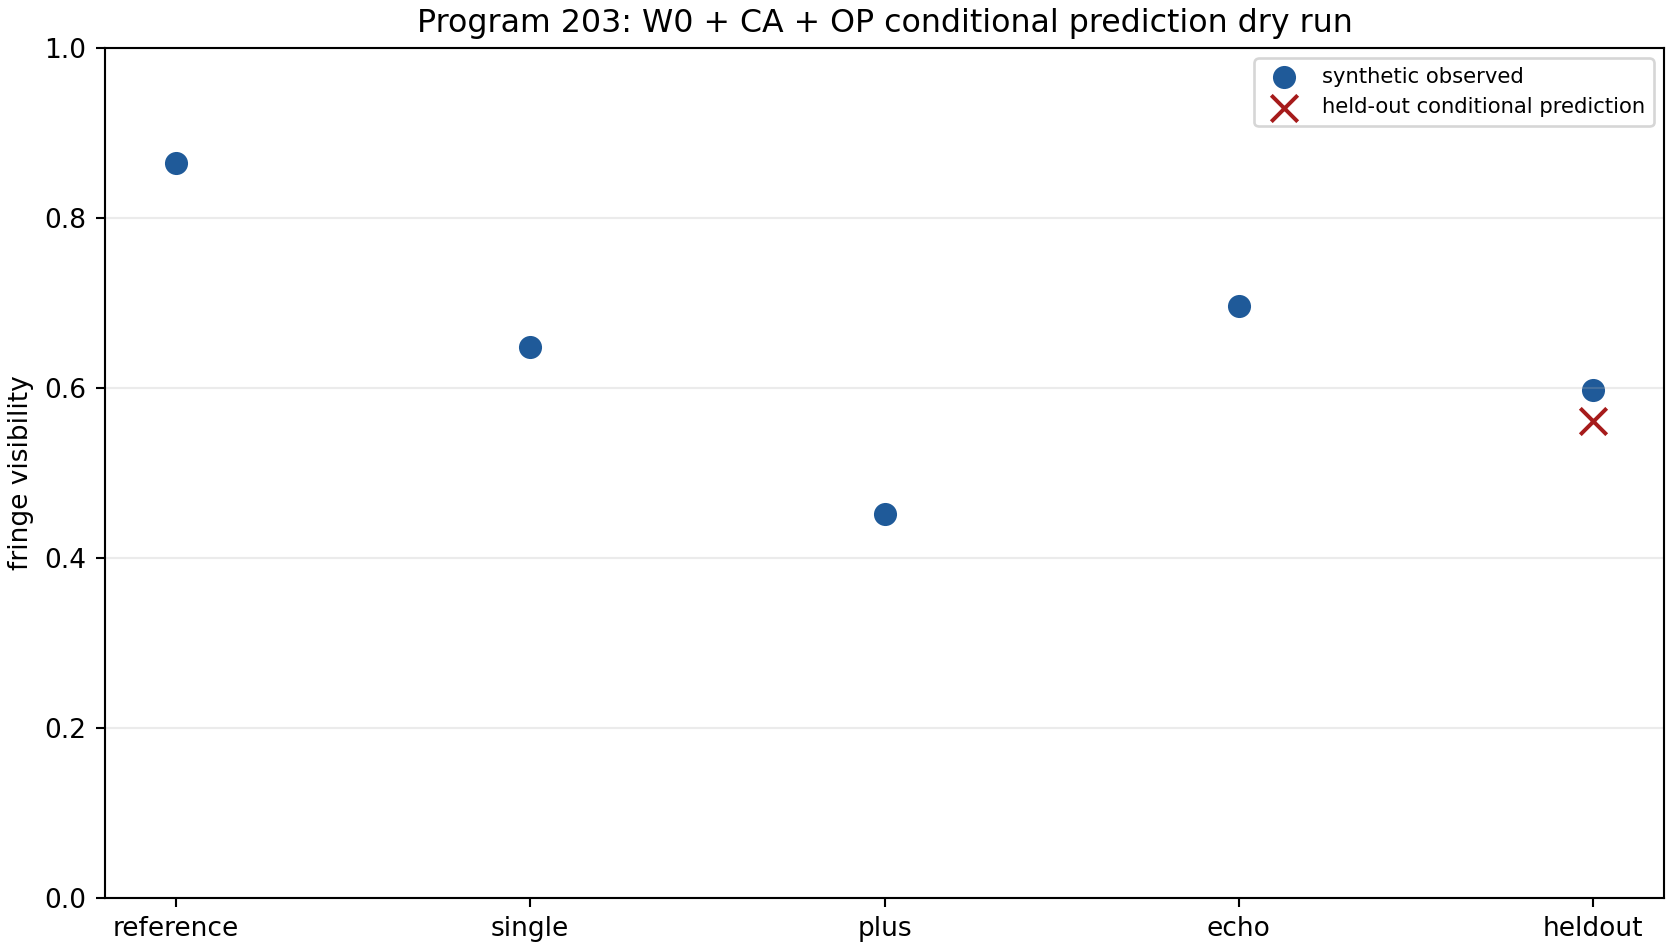
\includegraphics[width=0.94\textwidth]{FIN_Programs_191_203_Reference_Process_Prediction_Figures/program203_conditional_prediction.png}
\caption{A held-out visibility is predicted in an explicit W0 plus CA plus OP synthetic dry run.}
\end{figure}

\section{Verdict}

\textbf{Conditional, strong synthetic method evidence.} The complete \(W_0+\mathrm{CA}+\mathrm{OP}\) path can generate a held-out numerical prediction with every imported object visible. Because Program 202 did not admit an independent external bundle, this is a pipeline dry run, not an empirical FIN prediction.

\par\medskip\hrule\medskip

\chapter{Cross-program synthesis}

\section{The missing operational object is not one scalar}

The completed programs support the following typed structure:

\[
\mathfrak O
=
(\mathcal A,\omega,\mathcal P,\mathcal I,\Upsilon,
\mathcal E,\mathcal M,\mathcal D,\mathcal R,\tau_\ast).
\]

Here:

\begin{itemize}
\item 
\(\mathcal A\) is the observable algebra;

\item 
\(\omega\) is a state, including its central measure;

\item 
\(\mathcal P\) is a preparation family;

\item 
\(\mathcal I\) is an intervention family;

\item 
\(\Upsilon\) is a process tensor or operational equivalence class;

\item 
\(\mathcal E\) is an environment representation modulo dilation equivalence;

\item 
\(\mathcal M\) is a POVM or instrument;

\item 
\(\mathcal D\) is detector response and calibration;

\item 
\(\mathcal R\) is a persistent ordered record;

\item 
\(\tau_\ast\) is a conditional clock section.

\end{itemize}

The spectral generator \(A\) is necessary inside this structure but does not determine the remaining entries.

\section{State, scale, and environment are different quotient problems}

\begin{center}
\begingroup\small
\setlength{\tabcolsep}{3.5pt}
\renewcommand{\arraystretch}{1.16}
\begin{longtable}{@{}p{0.213\textwidth}p{0.328\textwidth}p{0.319\textwidth}@{}}
\toprule
\textbf{Layer} & \textbf{Symmetry or equivalence} & \textbf{Missing selection} \\
\midrule
\endhead
state & inner unitaries and central decomposition & central probability measure \\
compression & positive length rescaling & representative or physical length \\
environment & dilation and finite operational equivalence & microscopic model, if meaningful \\
phase & analytic/\allowbreak{}naturality class & origin-bearing source law \\
experiment & record equivalence and provenance & independent admissible dataset \\
\bottomrule
\end{longtable}
\endgroup
\end{center}

Trying to replace all five by one constant would erase their different domains and transformation laws.

\section{Observer paradox}

The same operator can generate both wave and diffusion dynamics without contradiction:

\[
U_t=e^{-itA},
\qquad
P_t=e^{-tA}.
\]

The observer paradox arises only if \(P_t\) is silently called collapse or measurement. In the operational model:

\begin{itemize}
\item 
\(U_t\) is system amplitude evolution;

\item 
\(P_t\) is a classical or Euclidean comparison semigroup;

\item 
measurement probabilities require a state and POVM;

\item 
memory requires a multi-time process;

\item 
apparatus response requires a detector channel;

\item 
observation requires a persistent record.

\end{itemize}

Programs 198, 199, 202, and 203 explicitly construct these distinctions.

\section{Information versus physics}

The dimensionless informational core can support exact spectral and operational probability structure. It does not turn Shannon information into thermodynamic entropy, seconds, joules, or metres without conversion data.

Program 201 shows that meaningful pre-clock predictions exist: they are projective spectral invariants. Program 203 shows how a physical-looking prediction can be produced after a clock and apparatus are supplied. The distinction is mathematical, not philosophical.

\par\medskip\hrule\medskip

\chapter{Falsification matrix}

\begin{center}
\begingroup\small
\setlength{\tabcolsep}{3.5pt}
\renewcommand{\arraystretch}{1.16}
\begin{longtable}{@{}p{0.229\textwidth}p{0.289\textwidth}p{0.124\textwidth}p{0.219\textwidth}@{}}
\toprule
\textbf{Proposal} & \textbf{Destructive test} & \textbf{Result} & \textbf{Surviving statement} \\
\midrule
\endhead
normalized trace is the unique state & non-simple direct sum & falsified & unique only blockwise \\
\(\beta=1\) is strict & positive-scale quotient & falsified & valid gauge representative \\
scale quotient completes bridge & compare \((\eta,\nu,\phi)\) & falsified & invariant mismatch remains \\
fractional certificate is finished & one-engine dependency gate & falsified & partial bounds remain \\
Lean formalization is compiled & local toolchain audit & falsified & source supplied, uncompiled \\
scalar \(M\) is complete & equal-\(M\) target & falsified & analytic AU cone is complete \\
nominal record count is iid size & regenerative chain & falsified & use observed refresh count \\
marginal features detect memory & multiset-preserving sort & falsified & order features required \\
two visibilities identify process + blur & Jacobian rank & falsified & echo gives minimal rank three \\
one channel identifies environment & two phase laws, same \(\gamma\) & falsified & identify operational quotient \\
analytic map sources strict phase & naturality/\allowbreak{}target-code audit & falsified & no accepted source class \\
raw gap is prediction & \(10^{12}\) scale orbit & falsified & projective ratios survive \\
synthetic complete metadata is experiment & independent-boundary gate & falsified & dry-run only \\
dry-run prediction validates FIN physics & external gate & falsified & conditional pipeline works \\
\bottomrule
\end{longtable}
\endgroup
\end{center}

\par\medskip\hrule\medskip

\chapter{Relation to established mathematics}

\section{Operator algebras}

Program 191 is a finite-dimensional instance of the distinction between states on simple matrix factors and states on algebras with nontrivial centre. The FIN-specific content is the dimension vector and the exact interpretation of \(9/5\) versus \(17/9\).

\section{Resource conversion}

Program 195 is an application and specialization of the Alberti--Uhlmann two-state transformation theorem. Its new contribution in this research sequence is the explicit reduction of the reflection-covariant boundary to three finite candidate points and its reconciliation with the previous Choi optimization.

\section{Empirical processes and mixing}

Program 196 uses regeneration to reduce a declared dependent acquisition class to conditional iid samples and then applies the DKW inequality. It does not pretend that DKW holds for arbitrary mixing records.

\section{Process tensors and quantum networks}

Programs 198 and 199 use the operational principle that multi-time processes are identified by interventions, not by a single reduced trajectory. The minimal three-contrast theorem is specific to the declared Gaussian dephasing-plus-blur family.

\section{Topological groups and transcendence}

Program 200 combines the classification of continuous circle-group endomorphisms with transcendence of the exponential of a nonzero algebraic number. It strengthens the earlier algebraic functional-calculus obstruction by adding a naturality condition.

\par\medskip\hrule\medskip

\chapter{Failed approaches and open obligations}

\section{Central state selection}

The strongest symmetry used in Program 191 does not exchange inequivalent simple blocks. A unique state requires one of:

\begin{itemize}
\item 
an explicit central probability measure;

\item 
a declared representation trace;

\item 
a Morita or categorical principle;

\item 
a physical preparation law.

\end{itemize}

Selecting the desired expectation first and solving for \(a\) is receiver fitting, not a source theorem.

\section{Rigorous numerics}

The Program 193 obstruction is infrastructural, not mathematical. The next attempt must provide a reproducible directed-rounding environment. Repeating ordinary floating-point estimates cannot close the certificate.

\section{Proof assistant}

The Program 194 source must be compiled against a pinned Lean and Mathlib version. Until then it is a formalization candidate, not machine-checked evidence.

\section{External experiment}

The synthetic bundle demonstrates format and analysis only. The next empirical step requires an independently sourced record whose preparation, apparatus, memory calibration, units, control, license, and hashes are genuinely documented.

\par\medskip\hrule\medskip

\chapter{Recommended Programs 204--216}

The following thirteen programs are ranked by expected scientific information gain. Their success criteria are deliberately finite.

\section{Priority 1 --- Program 204: Morita-natural central measure}

Classify state assignments under stronger categorical maps: direct sums, matrix amplification, Morita equivalence, and specified coarse-graining channels. Determine whether any noncircular axiom uniquely selects uniform central weight or represented-space trace.

\textbf{Success:} a uniqueness theorem with explicit hypotheses.\\
\textbf{Stop rule:} if different admissible functors yield \(9/5\) and \(17/9\), publish the independence theorem.

\section{Priority 2 --- Program 205: eta renormalization cocycle}

Attack one bridge atom only: whether a target-independent semigroup or renormalization cocycle can change the legacy damping exponent \(1\) into \(9/5\) while respecting the Program 192 quotient.

\textbf{Success:} an explicit cocycle law sourcing \(\eta=9/5\).\\
\textbf{Stop rule:} receiver interpolation or target subtraction is rejection.

\section{Priority 3 --- Program 206: reproducible Arb certificate}

Supply a pinned container or local environment with Arb/\allowbreak{}python-flint. Move all five fractional-symbol obligations into the same directed-rounding engine.

\textbf{Success:} formal width below 0.03 or a formal lower obstruction.\\
\textbf{Stop rule:} no mixed ordinary-float/\allowbreak{}ball promotion.

\section{Priority 4 --- Program 207: compiled Dirichlet library}

Pin Lean and Mathlib, repair any source errors, and compile the general Dirichlet identity, positivity, constant kernel, unitary group, and heat positivity/\allowbreak{}stochasticity.

\textbf{Success:} clean machine compilation with a reproducible lock file.\\
\textbf{Stop rule:} do not replace propositions by Boolean assertions.

\section{Priority 5 --- Program 208: tensor conversion and catalysis}

Extend Program 195 to two copies or a catalyst. Search for catalytic conversion outside the one-copy reflection cone and derive necessary trace-norm constraints.

\textbf{Success:} an explicit catalyst or a no-catalysis theorem in a finite class.

\section{Priority 6 --- Program 209: hidden-refresh confidence sequences}

Remove observed refresh flags. Construct a sequential confidence procedure using an estimable minorization, coupling, or martingale condition.

\textbf{Success:} finite-sample coverage under a fully observable acquisition assumption weaker than recorded regeneration.

\section{Priority 7 --- Program 210: sequential temporal conformal detector}

Replace the fixed Mahalanobis threshold by online conformal or e-value calibration. Challenge regime changes, long memory, detector resets, and adversarial multiset-preserving reorderings.

\textbf{Success:} time-uniform false-alarm control in the declared null class.

\section{Priority 8 --- Program 211: finite-shot process confidence region}

Put binomial phase-scan likelihoods around Program 198. Derive a confidence region for \((b,v,c)\) respecting

\[
b\in[0,1],
\qquad
v\ge0,
\qquad
|c|\le v.
\]

\textbf{Success:} finite-shot coverage and a power calculation for memory.

\section{Priority 9 --- Program 212: environment moment bounds}

Given finitely many measured characteristic values, solve the associated trigonometric moment problem. Bound unmeasured visibilities without choosing one microscopic phase law.

\textbf{Success:} sharp semidefinite upper and lower bounds.

\section{Priority 10 --- Program 213: formal phase-source no-go}

Formalize the continuous-endomorphism and algebraic-functional-calculus obstructions. Extend the audit to measurable homomorphisms and origin-bearing cocycles.

\textbf{Success:} one theorem covering all repository-admissible natural phase operations, or one genuine counterexample with source provenance.

\section{Priority 11 --- Program 214: scale-free falsification protocol}

Choose one projective spectral observable from Program 201 and preregister a test that requires no physical scale fit.

\textbf{Success:} a frozen dimensionless prediction and exclusion rule independent of \(c\).

\section{Priority 12 --- Program 215: independent experimental bundle}

Acquire or document one external record passing all eleven Program 202 fields. Generator and evaluator must be independent, and license and hashes must be frozen before analysis.

\textbf{Success:} the intake validator returns 11/\allowbreak{}11 and source class external.

\section{Priority 13 --- Program 216: first external conditional prediction}

Only after Program 215 passes, freeze one \(W_0+\mathrm{CA}+\mathrm{OP}\) prediction, estimate nuisance parameters on a training partition, and test a held-out partition.

\textbf{Success:} a preregistered residual or likelihood score on independent data. The result remains conditional unless CA and OP are separately sourced by theory.

\section{Quantitative ranking}

\begin{center}
\begingroup\small
\setlength{\tabcolsep}{3.5pt}
\renewcommand{\arraystretch}{1.16}
\begin{longtable}{@{}p{0.160\textwidth}p{0.280\textwidth}p{0.420\textwidth}@{}}
\toprule
\textbf{Rank} & \textbf{Program} & \textbf{Estimated probability of decisive progress} \\
\midrule
\endhead
1 & 204 & 0.88 \\
2 & 211 & 0.86 \\
3 & 212 & 0.84 \\
4 & 207 & 0.82 \\
5 & 210 & 0.80 \\
6 & 205 & 0.76 \\
7 & 209 & 0.74 \\
8 & 206 & 0.72 \\
9 & 214 & 0.70 \\
10 & 208 & 0.66 \\
11 & 213 & 0.64 \\
12 & 215 & 0.42 \\
13 & 216 & 0.30 \\
\bottomrule
\end{longtable}
\endgroup
\end{center}

The external programs rank lower only because their prerequisites are not currently present. A rigorous independence or no-go theorem counts as decisive progress.

\par\medskip\hrule\medskip

\chapter{Final conclusion}

Programs 191--203 identify the current mathematical boundary more sharply than a search for another fitted number could.

The finite spectral generator is a genuine common engine. It supports exact Dirichlet energy, wave evolution, heat evolution, Green response, scale-free observables, and finite operational probability models.

However:

\begin{itemize}
\item 
the state on a non-simple algebra requires a central measure;

\item 
positive compression requires a scale section;

\item 
phase conversion requires an origin-bearing source law;

\item 
environmental dynamics are identified only modulo an operational quotient;

\item 
process memory requires interventions;

\item 
apparatus response requires calibration;

\item 
physics requires an independent record with units and provenance.

\end{itemize}

These missing objects can be constructed conditionally and tested. Programs 198, 202, and 203 demonstrate the full logic without concealing imports. The right next goal is not to call those imports strict FIN, but to either derive them, bound their operational equivalence classes, or test conditional predictions on admissible external data.

The deepest interpretation surviving this round is:

\textbf{FIN is a dimensionless spectral-information core whose route to physics is an operational quotient-and-section problem. The core already determines nontrivial dynamics and conversion geometry, but states, scale, environment, apparatus, and empirical records are independent typed objects until a theorem or experiment fixes them.}

\par\medskip\hrule\medskip

\chapter{Selected mathematical references}

\begin{enumerate}
\item 
P. M. Alberti and A. Uhlmann, \emph{Stochasticity and Partial Order: Doubly Stochastic Maps and Unitary Mixing}, D. Reidel, 1982.

\item 
W. F. Stinespring, "Positive functions on C*-algebras," \emph{Proceedings of the American Mathematical Society} 6 (1955), 211--216.

\item 
A. Dvoretzky, J. Kiefer, and J. Wolfowitz, "Asymptotic minimax character of the sample distribution function and of the classical multinomial estimator," \emph{Annals of Mathematical Statistics} 27 (1956), 642--669.

\item 
P. Massart, "The tight constant in the Dvoretzky--Kiefer--Wolfowitz inequality," \emph{Annals of Probability} 18 (1990), 1269--1283.

\item 
E. B. Davies, \emph{Heat Kernels and Spectral Theory}, Cambridge University Press, 1989.

\item 
R. Bhatia, \emph{Matrix Analysis}, Springer, 1997.

\item 
F. A. Pollock et al., "Operational Markov condition for quantum processes," \emph{Physical Review Letters} 120 (2018), 040405.

\item 
G. Chiribella, G. M. D'Ariano, and P. Perinotti, "Theoretical framework for quantum networks," \emph{Physical Review A} 80 (2009), 022339.

\end{enumerate}

\par\medskip\hrule\medskip

\chapter{Archival statement}

Suggested citation:

\.Zuchowski, K. (2026). \emph{FIN Programs 191--203: Reference States, Operational Quotients, and Conditional Prediction} (FIN Research Monograph, Release 10.18; Version 1.0.0) [Preprint]. Zenodo.


\clearpage
\chapter*{Release reproducibility}
\addcontentsline{toc}{chapter}{Release reproducibility}
\begin{Verbatim}[fontsize=\small]
python3 fin_programs_191_203_reference_process_prediction.py
python3 -m unittest -v \
  test_fin_programs_191_203_reference_process_prediction.py
\end{Verbatim}

Machine-readable results are stored in
\path{FIN_Programs_191_203_Reference_Process_Prediction_Results.json}.
The release also contains the frozen order-sensitive protocol, the synthetic
operational dry-run bundle, the finite Lean source, sixty-five tests and
thirteen figures.

\medskip
\noindent\textbf{Suggested citation:}

\.Zuchowski, K. (2026). \emph{FIN Programs 191--203: Reference States,
Operational Quotients, and Conditional Prediction}
(FIN Research Monograph, Release 10.18; Version 1.0.0) [Preprint]. Zenodo.
\end{document}
